%. Author = ktarrant
%. Date = 3/27/23

% Preamble
\documentclass[11pt]{article}

% Packages
\usepackage{amsmath}
\usepackage[T1]{fontenc}%
\usepackage[utf8]{inputenc}%
\usepackage{lmodern}%
\usepackage{textcomp}%
\usepackage{lastpage}%
\usepackage{longtable}%
\usepackage{graphicx}
\usepackage{wrapfig}
\usepackage{mdframed}
\usepackage[default]{gillius}
\usepackage[dvipsnames]{xcolor}
\usepackage{colortbl}
\usepackage{ulem}
\usepackage{multirow}
\usepackage{titlesec}
\graphicspath{ {./imgs/} }

\title{Pokemon Revolution Online Full Walkthrough}

\definecolor{LightColor}{HTML}{DDEAEE}
\definecolor{DarkColor}{HTML}{42445A}
\definecolor{MedColor}{HTML}{8CACD0}
\definecolor{GroundColor}{HTML}{D7B5A1}
\definecolor{WaterColor}{HTML}{22B2EA}


\mdfdefinestyle{PokemonSpotlight}{
    linecolor=black,
    outerlinewidth=2pt,
    %roundcorner=20pt,
    innertopmargin=4pt,
    innerbottommargin=4pt,
    innerrightmargin=4pt,
    innerleftmargin=4pt,
    leftmargin = 4pt,
    rightmargin = 4pt,
    backgroundcolor=MedColor!50!white
}


% Document
\begin{document}
\pagecolor{LightColor}

\maketitle

\tableofcontents

\section{Johto}\label{sec:johto}

Part 1 - Intro, New Bark Town, Routes 29 and 30, Cherrygrove City, Route 31
Part 2 - Violet City, Sprout Tower, Route 32, Union Cave, Route 33, Azalea Town
Part 3 - Slowpoke Well, Azalea Town, Ilex Forest, Route 34
Part 4 - Goldenrod City, Route 35
Part 5 - National Park, Routes 36 and 37, Ecruteak City, Burned Tower
Part 6 - Ecruteak Gym, Union Cave, Routes 38 and 39, Olivine City, Route 40
Part 7 - Route 41, Cianwood City, Olivine City, Route 47, Cliff Cave, Route 48, Safari Zone Gate
Part 8 - Route 42, Mahogany Town, Route 43, Lake of Rage, Mahogany Town
Part 9 - Lake of Rage, Goldenrod City
Part 10 - Route 44, Ice Path, Blackthorn City
Part 11 - Route 45, Dark Cave, Route 46, Dragon's Den
Part 12 - Mt. Mortar, New Bark Town, Ecruteak City, Bell Tower
Part 13 - Whirl Islands, Ruins of Alph

\subsection{Walkthrough}\label{subsec:walkthrough}

\subsubsection{New Bark Town}%
\label{ssubsec:NewBarkTown}%

%
\input{routes/Johto/New_Bark_Town/Wild_Pokémon_(Headbuttable_Trees)}%
\subsubsection{Route 29}%
\label{ssubsec:Route29}%

%
\input{routes/Johto/Route_29/Wild_Pokémon_(Headbuttable_Trees)}%
\begin{longtable}{|| l l l l ||}%
\hline%
&Oran Berry&x 1{-}3&3 days.\\%
\multicolumn{4}{||m{\textwidth}||}{Berry tree in the north-west part.}%
\hline%
\endhead%
\hline%
\caption{Items in Route 29}%
\label{tab:Route29Items}%
\end{longtable}%
\input{routes/Johto/Route_29/Wild_Pokémon_(Land)}%
\subsubsection{Route 30}%
\label{ssubsec:Route30}%

%
\input{routes/Johto/Route_30/Wild_Pokémon_(Headbuttable_Trees)}%
\begin{longtable}{|| l l l l ||}%
\hline%
&TM18 — Counter&x 1&Not respawnable\\%
\multicolumn{4}{||m{\textwidth}||}{Behind the Camper in the north part of the route, hidden behind a tree on the large ledge. The Camper needs to move out of the way, meaning it can only be obtained once you defeat the Camper.}%
\hline%
&Full Heal&x 1&Not respawnable\\%
\multicolumn{4}{||m{\textwidth}||}{Beyond the water in the south-east corner of the route.}%
\hline%
&Oran Berry&x 1{-}3&3 days\\%
\multicolumn{4}{||m{\textwidth}||}{Berry Tree next to the southmost house.}%
\hline%
&Pecha Berry&x 1{-}3&3 day\\%
\multicolumn{4}{||m{\textwidth}||}{Berry Tree close to the northmost house.}%
\hline%
\endhead%
\hline%
\caption{Items in Route 30}%
\label{tab:Route30Items}%
\end{longtable}%
\input{routes/Johto/Route_30/Wild_Pokémon_(Land)}%
\subsubsection{Cherrygrove City}%
\label{ssubsec:CherrygroveCity}%

%
\input{routes/Johto/Cherrygrove_City/Wild_Pokémon_(Headbuttable_Trees)}%
\input{routes/Johto/Cherrygrove_City/Wild_Pokémon_(Water)}%
\begin{longtable}{|| l l l l ||}%
\hline%
&Pokéball&&\\%
\hline%
&Potion&&\\%
\hline%
&Antidote&&\\%
\hline%
&Paralyze Heal&&\\%
\hline%
&Awakening&&\\%
\hline%
&Burn Heal&&\\%
\hline%
&Ice Heal&&\\%
\hline%
&Ether&&\\%
\hline%
&Repel&&\\%
\hline%
&Escape Rope&&\\%
\hline%
\endhead%
\hline%
\caption{Items in Cherrygrove City}%
\label{tab:CherrygroveCityItems}%
\end{longtable}%
\subsubsection{Route 31}%
\label{ssubsec:Route31}%

%
\input{routes/Johto/Route_31/Wild_Pokémon_(Headbuttable_Trees)}%
\begin{longtable}{|| l l l l ||}%
\hline%
&Leppa Berry&x 1{-}3&3 day\\%
\multicolumn{4}{||m{\textwidth}||}{Berry Tree near the pond.}%
\hline%
&Persim Berry&x 1{-}3&3 day\\%
\multicolumn{4}{||m{\textwidth}||}{Berry Tree near the pond.}%
\hline%
\endhead%
\hline%
\caption{Items in Route 31}%
\label{tab:Route31Items}%
\end{longtable}%
\input{routes/Johto/Route_31/Wild_Pokémon_(Land)}%
\subsubsection{Violet City}%
\label{ssubsec:VioletCity}%

%
\input{routes/Johto/Violet_City/Wild_Pokémon_(Headbuttable_Trees)}%
\input{routes/Johto/Violet_City/Wild_Pokémon_(Water)}%
\begin{longtable}{|| l l l l ||}%
\hline%
\endhead%
\hline%
\caption{Items in Violet City}%
\label{tab:VioletCityItems}%
\end{longtable}%
\subsubsection{Sprout Tower}%
\label{ssubsec:SproutTower}%

%
\begin{longtable}{|| l l l l ||}%
\hline%
&Potion&x 1&Not respawnable\\%
\multicolumn{4}{||m{\textwidth}||}{North-west corner of Sprout Tower F2.}%
\hline%
&Paralyze Heal&x 1&Not respawnable\\%
\multicolumn{4}{||m{\textwidth}||}{Further to the east before climbing the ladder to F3 in Sprout Tower F2.}%
\hline%
&Escape Rope&x 1&Not respawnable\\%
\multicolumn{4}{||m{\textwidth}||}{Next to the Master in Sprout Tower F3.}%
\hline%
\endhead%
\hline%
\caption{Items in Sprout Tower}%
\label{tab:SproutTowerItems}%
\end{longtable}%
\subsubsection{Route 32}%
\label{ssubsec:Route32}%

%
\input{routes/Johto/Route_32/Wild_Pokémon_(Headbuttable_Trees)}%
\input{routes/Johto/Route_32/Wild_Pokémon_(Water)}%
\begin{longtable}{|| l l l l ||}%
\hline%
\endhead%
\hline%
\caption{Items in Route 32}%
\label{tab:Route32Items}%
\end{longtable}%
\input{routes/Johto/Route_32/Wild_Pokémon_(Land)}%
\subsubsection{Union Cave}%
\label{ssubsec:UnionCave}%

%
\begin{longtable}{|| l l l l ||}%
\hline%
&Super Potion&x 1&Not respawnable\\%
\multicolumn{4}{||m{\textwidth}||}{In a eastern corner of 1F, close to the Picnicker.}%
\hline%
&Great Ball&x 1&Not respawnable\\%
\multicolumn{4}{||m{\textwidth}||}{On-ground dead end on the far west of the Picnicker in 1F, initially garded by an Old man.}%
\hline%
&Pokeball&x 1&Not respawnable\\%
\multicolumn{4}{||m{\textwidth}||}{Hidden item. On the only rock in the south-west corner of B1F. Requires Surf to reach this part of B1F.}%
\hline%
\endhead%
\hline%
\caption{Items in Union Cave}%
\label{tab:UnionCaveItems}%
\end{longtable}%
\subsubsection{Route 33}%
\label{ssubsec:Route33}%

%
\input{routes/Johto/Route_33/Wild_Pokémon_(Headbuttable_Trees)}%
\input{routes/Johto/Route_33/Wild_Pokémon_(Land)}%
\subsubsection{Azalea Town}%
\label{ssubsec:AzaleaTown}%

%
\input{routes/Johto/Azalea_Town/Wild_Pokémon_(Headbuttable_Trees)}%
\subsubsection{Slowpoke Well}%
\label{ssubsec:SlowpokeWell}%

%
\begin{longtable}{|| l l l l ||}%
\hline%
&Pokeball&x 1&3 Days\\%
\multicolumn{4}{||m{\textwidth}||}{From the Diggable Patches in the first floor..}%
\hline%
&Ghost Gem&x 1&3 Days\\%
\multicolumn{4}{||m{\textwidth}||}{From the Diggable Patches in the first floor..}%
\hline%
&Nugget&x 1&3 Days\\%
\multicolumn{4}{||m{\textwidth}||}{From the Diggable Patches in the first floor..}%
\hline%
&Soda Pop&x 1&3 Days\\%
\multicolumn{4}{||m{\textwidth}||}{From the Diggable Patches in the first floor..}%
\hline%
&Fast Ball&x 1&3 Days\\%
\multicolumn{4}{||m{\textwidth}||}{From the Diggable Patches in the first floor..}%
\hline%
&Nest Ball&x 1&3 Days\\%
\multicolumn{4}{||m{\textwidth}||}{From the Diggable Patches in the first floor..}%
\hline%
&Leftovers&x 1&3 Days\\%
\multicolumn{4}{||m{\textwidth}||}{From the Diggable Patches in the first floor..}%
\hline%
&Calcium&x 1&3 Days\\%
\multicolumn{4}{||m{\textwidth}||}{From the Diggable Patches in the first floor..}%
\hline%
&Root Fossil&x 1&3 Days\\%
\multicolumn{4}{||m{\textwidth}||}{From the Diggable Patches in the first floor..}%
\hline%
&Claw Fossil&x 1&3 Days\\%
\multicolumn{4}{||m{\textwidth}||}{From the Diggable Patches in the first floor..}%
\hline%
&Insect Plate&x 1&3 Days\\%
\multicolumn{4}{||m{\textwidth}||}{From the Diggable Patches in the first floor..}%
\hline%
&Pokeball&x 1&3 Days\\%
\multicolumn{4}{||m{\textwidth}||}{From the Diggable Patches in L1.}%
\hline%
&Grass Gem&x 1&3 Days\\%
\multicolumn{4}{||m{\textwidth}||}{From the Diggable Patches in L1.}%
\hline%
&Potion&x 1&3 Days\\%
\multicolumn{4}{||m{\textwidth}||}{From the Diggable Patches in L1.}%
\hline%
&Paralyze Heal&x 1&3 Days\\%
\multicolumn{4}{||m{\textwidth}||}{From the Diggable Patches in L1.}%
\hline%
&Dusk Stone&x 1&3 Days\\%
\multicolumn{4}{||m{\textwidth}||}{From the Diggable Patches in L1.}%
\hline%
&Friend Ball&x 1&3 Days\\%
\multicolumn{4}{||m{\textwidth}||}{From the Diggable Patches in L1.}%
\hline%
&Leftovers&x 1&3 Days\\%
\multicolumn{4}{||m{\textwidth}||}{From the Diggable Patches in L1.}%
\hline%
&Protein&x 1&3 Days\\%
\multicolumn{4}{||m{\textwidth}||}{From the Diggable Patches in L1.}%
\hline%
&Root Fossil&x 1&3 Days\\%
\multicolumn{4}{||m{\textwidth}||}{From the Diggable Patches in L1.}%
\hline%
&Claw Fossil&x 1&3 Days\\%
\multicolumn{4}{||m{\textwidth}||}{From the Diggable Patches in L1.}%
\hline%
&Iron Plate&x 1&3 Days\\%
\multicolumn{4}{||m{\textwidth}||}{From the Diggable Patches in L1.}%
\hline%
\endhead%
\hline%
\caption{Items in Slowpoke Well}%
\label{tab:SlowpokeWellItems}%
\end{longtable}%
\subsubsection{Ilex Forest}%
\label{ssubsec:IlexForest}%

%
\input{routes/Johto/Ilex_Forest/Wild_Pokémon_(Headbuttable_Trees)}%
\input{routes/Johto/Ilex_Forest/Wild_Pokémon_(Water)}%
\input{routes/Johto/Ilex_Forest/Wild_Pokémon_(Land)}%
\subsubsection{Route 34}%
\label{ssubsec:Route34}%

%
\input{routes/Johto/Route_34/Wild_Pokémon_(Headbuttable_Trees)}%
\input{routes/Johto/Route_34/Wild_Pokémon_(Water)}%
\begin{longtable}{|| l l l l ||}%
\hline%
&Soft Sand&x 1&20 days\\%
\multicolumn{4}{||m{\textwidth}||}{At the end of the surf path, along with the Herb sisters.}%
\hline%
\endhead%
\hline%
\caption{Items in Route 34}%
\label{tab:Route34Items}%
\end{longtable}%
\input{routes/Johto/Route_34/Wild_Pokémon_(Land)}%
\subsubsection{Goldenrod City}%
\label{ssubsec:GoldenrodCity}%

%
\begin{longtable}{|| l l l l ||}%
\hline%
&TM46 — Psywave&x 1&9 days\\%
\multicolumn{4}{||m{\textwidth}||}{At the north extremity of Underground Path.}%
\hline%
&Full Heal&x 1&4 days\\%
\multicolumn{4}{||m{\textwidth}||}{Behind the tree at the start of the eastern path in Underground Path.}%
\hline%
&Max Ether&x 2&11 days\\%
\multicolumn{4}{||m{\textwidth}||}{Behind the southmost tree in Underground Path.}%
\hline%
&Antidote&x 2&7 days\\%
\multicolumn{4}{||m{\textwidth}||}{Behind the eastmost tree in Underground Path.}%
\hline%
&Revive&x 1&3{-}9 days\\%
\multicolumn{4}{||m{\textwidth}||}{In the path west of the stairs in Underground Warehouse.}%
\hline%
&Super Potion&x 1{-}2&4{-}5 days\\%
\multicolumn{4}{||m{\textwidth}||}{At the end of the path west of the stairs in Underground Warehouse.}%
\hline%
&Max Potion&x 1&3{-}8 days\\%
\multicolumn{4}{||m{\textwidth}||}{Between boxes in the southern part of Underground Warehouse.}%
\hline%
&Antidote&x 1&2{-}3 days\\%
\multicolumn{4}{||m{\textwidth}||}{Immediately next to the west exit in Underground Warehouse.}%
\hline%
&Great Ball&x 2{-}5&4{-}7 days\\%
\multicolumn{4}{||m{\textwidth}||}{Hidden Item. In the trash placed in the northwest corner of Underground Warehouse.}%
\hline%
&TM62 — Taunt&x 1&18 days\\%
\multicolumn{4}{||m{\textwidth}||}{In the final room of the lever puzzle in Underground Basement.}%
\hline%
&BrightPowder&x 1&5{-}12 days\\%
\multicolumn{4}{||m{\textwidth}||}{Hidden Item. In the trash can placed in the southeast corner of Underground Basement.}%
\hline%
&Miracle Seed&x 1&10 days\\%
\multicolumn{4}{||m{\textwidth}||}{Hidden Item. In the jar between the two exits of Underground Basement.}%
\hline%
\endhead%
\hline%
\caption{Items in Goldenrod City}%
\label{tab:GoldenrodCityItems}%
\end{longtable}%
\subsubsection{Route 35}%
\label{ssubsec:Route35}%

%
\input{routes/Johto/Route_35/Wild_Pokémon_(Headbuttable_Trees)}%
\input{routes/Johto/Route_35/Wild_Pokémon_(Water)}%
\begin{longtable}{|| l l l l ||}%
\hline%
&Paralyze Heal&x 1&Not respawnable\\%
\multicolumn{4}{||m{\textwidth}||}{Partly hidden in the trees east of the two Firebreathers.}%
\hline%
&TM42 — Dream Eater&x 1&Not respawnable\\%
\multicolumn{4}{||m{\textwidth}||}{In the grassy path behind the fence, close to Lass Darlene.}%
\hline%
&Lum Berry&x 1{-}3&3 days\\%
\multicolumn{4}{||m{\textwidth}||}{Berry tree past the water. Requires Surf.}%
\hline%
&Nugget&x 1&Not respawnable\\%
\multicolumn{4}{||m{\textwidth}||}{Hidden item. Two tiles south of the berry tree. Requires Surf.}%
\hline%
\endhead%
\hline%
\caption{Items in Route 35}%
\label{tab:Route35Items}%
\end{longtable}%
\input{routes/Johto/Route_35/Wild_Pokémon_(Land)}%
\subsubsection{National Park}%
\label{ssubsec:NationalPark}%

%
\begin{longtable}{|| l l l l ||}%
\hline%
\endhead%
\hline%
\caption{Items in National Park}%
\label{tab:NationalParkItems}%
\end{longtable}%
\input{routes/Johto/National_Park/Wild_Pokémon_(Land)}%
\subsubsection{Route 36}%
\label{ssubsec:Route36}%

%
\input{routes/Johto/Route_36/Wild_Pokémon_(Headbuttable_Trees)}%
\begin{longtable}{|| l l l l ||}%
\hline%
&Leppa Berry&x 1{-}3&3 Days\\%
\multicolumn{4}{||m{\textwidth}||}{Berry Tree immediately west of the intersection.}%
\hline%
&Sitrus Berry&x 1{-}4&3 Days\\%
\multicolumn{4}{||m{\textwidth}||}{Berry Tree immediately west of the intersection.}%
\hline%
\endhead%
\hline%
\caption{Items in Route 36}%
\label{tab:Route36Items}%
\end{longtable}%
\input{routes/Johto/Route_36/Wild_Pokémon_(Land)}%
\subsubsection{Route 37}%
\label{ssubsec:Route37}%

%
\begin{longtable}{|| l l l l ||}%
\hline%
&Magnet&x 1&Non respawnable\\%
\multicolumn{4}{||m{\textwidth}||}{Hidden Item. In the trash can nearby the south end of the route.}%
\hline%
&Ether&x 1&Non respawnable\\%
\multicolumn{4}{||m{\textwidth}||}{Hidden Item. Behind the closest tree to the Gentleman Jim.}%
\hline%
&Sun Stone&x 1&Non respawnable\\%
\multicolumn{4}{||m{\textwidth}||}{Hidden Item. On the small tree directly east of Gentleman Jim.}%
\hline%
&Pecha Berry&x 1{-}3&3 days\\%
\multicolumn{4}{||m{\textwidth}||}{Berry tree in the south-east part.}%
\hline%
&Chesto Berry&x 1{-}3&3 days\\%
\multicolumn{4}{||m{\textwidth}||}{Berry tree in the south-east part.}%
\hline%
&Cheri Berry&x 1{-}3&3 days\\%
\multicolumn{4}{||m{\textwidth}||}{Berry tree in the south-east part.}%
\hline%
\endhead%
\hline%
\caption{Items in Route 37}%
\label{tab:Route37Items}%
\end{longtable}%
\input{routes/Johto/Route_37/Wild_Pokémon_(Land)}%
\subsubsection{Ecruteak City}%
\label{ssubsec:EcruteakCity}%

%
\input{routes/Johto/Ecruteak_City/Wild_Pokémon_(Water)}%
\begin{longtable}{|| l l l l ||}%
\hline%
\endhead%
\hline%
\caption{Items in Ecruteak City}%
\label{tab:EcruteakCityItems}%
\end{longtable}%
\subsubsection{Burned Tower}%
\label{ssubsec:BurnedTower}%

%
\begin{longtable}{|| l l l l ||}%
\hline%
&Burn Heal&x 1&Not respawnable\\%
\multicolumn{4}{||m{\textwidth}||}{North-east corner of the Top floor.}%
\hline%
&Ether&x 1&Not respawnable\\%
\multicolumn{4}{||m{\textwidth}||}{Hidden Item. On the pile of debris closest to the ladder on Top floor.}%
\hline%
&TM115 — Shadow Claw&x 1&Not respawnable\\%
\multicolumn{4}{||m{\textwidth}||}{Immediately south of the ladder in the Bottom floor.}%
\hline%
&Burn Heal&x 1&Not respawnable\\%
\multicolumn{4}{||m{\textwidth}||}{North-west corner of the Bottom floor.}%
\hline%
&Ultra Ball&x 1&Not respawnable\\%
\multicolumn{4}{||m{\textwidth}||}{Middle south of the Bottom floor. Requires Rock Smash.}%
\hline%
&Revive&x 1&Not respawnable\\%
\multicolumn{4}{||m{\textwidth}||}{Hidden Item. On the teal rock on tile south of the first Rock Smash rock blocking the way in the Bottom floor.}%
\hline%
&Antidote&x 1&Not respawnable\\%
\multicolumn{4}{||m{\textwidth}||}{Hidden Item. On the third teal rock west from the large pillar in the north-east corner of the Bottom floor.}%
\hline%
&Nugget&x 1&Not respawnable\\%
\multicolumn{4}{||m{\textwidth}||}{Hidden Item. On the teal rock adjacent south of the pile of debris between the north and west stairs in Bottom floor. Requires Rock Smash.}%
\hline%
\endhead%
\hline%
\caption{Items in Burned Tower}%
\label{tab:BurnedTowerItems}%
\end{longtable}%
\input{routes/Johto/Burned_Tower/Wild_Pokémon_(Land)}%
\subsubsection{Route 38}%
\label{ssubsec:Route38}%

%
\input{routes/Johto/Route_38/Wild_Pokémon_(Headbuttable_Trees)}%
\begin{longtable}{|| l l l l ||}%
\hline%
&Max Potion&x 1&Not respawnable\\%
\multicolumn{4}{||m{\textwidth}||}{Middle north of the route, adjacent to Lass Dana.}%
\hline%
&Lum Berry&x 1{-}3&3 days\\%
\multicolumn{4}{||m{\textwidth}||}{Berry tree in the southwest of the route.}%
\hline%
&Oran Berry&x 1{-}5&3 days\\%
\multicolumn{4}{||m{\textwidth}||}{Berry tree in the southwest of the route.}%
\hline%
&HP Up&x 1&Not respawnable\\%
\multicolumn{4}{||m{\textwidth}||}{Hidden Item. Behind the trees directly south of the east gate.}%
\hline%
&Thunder Stone&x 1&Not respawnable\\%
\multicolumn{4}{||m{\textwidth}||}{Hidden Item. Behind the tree south-east of the berry trees in the south-west part of the route.}%
\hline%
\endhead%
\hline%
\caption{Items in Route 38}%
\label{tab:Route38Items}%
\end{longtable}%
\input{routes/Johto/Route_38/Wild_Pokémon_(Land)}%
\subsubsection{Route 39}%
\label{ssubsec:Route39}%

%
\begin{longtable}{|| l l l l ||}%
\hline%
&Moomoo Milk&x 1&Not respawnable\\%
\multicolumn{4}{||m{\textwidth}||}{Behind the Moo Moo Farm building.}%
\hline%
&PP Up&x 1&Not respawnable\\%
\multicolumn{4}{||m{\textwidth}||}{Hidden Item. On the southwest-most bush of the route.}%
\hline%
&Nugget&x 1&Not respawnable\\%
\multicolumn{4}{||m{\textwidth}||}{Hidden Item. On the lamppost next to the sentret near the south exit.}%
\hline%
\endhead%
\hline%
\caption{Items in Route 39}%
\label{tab:Route39Items}%
\end{longtable}%
\input{routes/Johto/Route_39/Wild_Pokémon_(Land)}%
\subsubsection{Olivine City}%
\label{ssubsec:OlivineCity}%

%
\input{routes/Johto/Olivine_City/Wild_Pokémon_(Water)}%
\begin{longtable}{|| l l l l ||}%
\hline%
\endhead%
\hline%
\caption{Items in Olivine City}%
\label{tab:OlivineCityItems}%
\end{longtable}%
\subsubsection{Route 40}%
\label{ssubsec:Route40}%

%
\input{routes/Johto/Route_40/Wild_Pokémon_(Water)}%
\begin{longtable}{|| l l l l ||}%
\hline%
&Hyper Potion&x 1&Not respawnable\\%
\multicolumn{4}{||m{\textwidth}||}{On the small island TubeGirl Sophie is on.}%
\hline%
\endhead%
\hline%
\caption{Items in Route 40}%
\label{tab:Route40Items}%
\end{longtable}%
\input{routes/Johto/Route_40/Wild_Pokémon_(Land)}%
\subsubsection{Route 41}%
\label{ssubsec:Route41}%

%
\input{routes/Johto/Route_41/Wild_Pokémon_(Water)}%
\subsubsection{Cianwood City}%
\label{ssubsec:CianwoodCity}%

%
\input{routes/Johto/Cianwood_City/Wild_Pokémon_(Water)}%
\subsubsection{Route 47}%
\label{ssubsec:Route47}%

%
\input{routes/Johto/Route_47/Wild_Pokémon_(Water)}%
\begin{longtable}{|| l l l l ||}%
\hline%
&Ultra Ball&x 1&Not respawnable\\%
\multicolumn{4}{||m{\textwidth}||}{Next to the Explosion tutor near the north end of the route.}%
\hline%
\endhead%
\hline%
\caption{Items in Route 47}%
\label{tab:Route47Items}%
\end{longtable}%
\input{routes/Johto/Route_47/Wild_Pokémon_(Land)}%
\subsubsection{Cliff Cave}%
\label{ssubsec:CliffCave}%

%
\subsubsection{Route 48}%
\label{ssubsec:Route48}%

%
\begin{longtable}{|| l l l l ||}%
\hline%
&PP Up&x 1&Not respawnable\\%
\multicolumn{4}{||m{\textwidth}||}{Inbetween ledges directly north from the southern entrance.}%
\hline%
\endhead%
\hline%
\caption{Items in Route 48}%
\label{tab:Route48Items}%
\end{longtable}%
\input{routes/Johto/Route_48/Wild_Pokémon_(Land)}%
\subsubsection{Route 42}%
\label{ssubsec:Route42}%

%
\begin{longtable}{|| l l l l ||}%
\hline%
&Ultra Ball&x 1&Not respawnable\\%
\multicolumn{4}{||m{\textwidth}||}{Hidden item. Between trees near the water in the south-east of the middle-south Mt. Mortar entrance.}%
\hline%
&Sitrus Berry&x 1{-}3&3 days\\%
\multicolumn{4}{||m{\textwidth}||}{Berry Tree near the middle north Mt. Mortar entrance.}%
\hline%
&Lum Berry&x 1{-}3&3 days\\%
\multicolumn{4}{||m{\textwidth}||}{Berry Tree near the middle north Mt. Mortar entrance.}%
\hline%
\endhead%
\hline%
\caption{Items in Route 42}%
\label{tab:Route42Items}%
\end{longtable}%
\subsubsection{Mahogany Town}%
\label{ssubsec:MahoganyTown}%

%
\begin{longtable}{|| l l l l ||}%
\hline%
&Pokeball&x 1&Not respawnable\\%
\multicolumn{4}{||m{\textwidth}||}{Hidden Item. On the well near the east exit.}%
\hline%
\endhead%
\hline%
\caption{Items in Mahogany Town}%
\label{tab:MahoganyTownItems}%
\end{longtable}%
\subsubsection{Route 43}%
\label{ssubsec:Route43}%

%
\begin{longtable}{|| l l l l ||}%
\hline%
&Leppa Berry&x 1{-}3&3 days\\%
\multicolumn{4}{||m{\textwidth}||}{Berry trees in the middle of the main path. There are two of them.}%
\hline%
\endhead%
\hline%
\caption{Items in Route 43}%
\label{tab:Route43Items}%
\end{longtable}%
\subsubsection{Lake of Rage}%
\label{ssubsec:LakeofRage}%

%
\input{routes/Johto/Lake_of_Rage/Wild_Pokémon_(Water)}%
\begin{longtable}{|| l l l l ||}%
\hline%
\endhead%
\hline%
\caption{Items in Lake of Rage}%
\label{tab:LakeofRageItems}%
\end{longtable}%
\input{routes/Johto/Lake_of_Rage/Wild_Pokémon_(Land)}%
\subsubsection{Route 44}%
\label{ssubsec:Route44}%

%
\input{routes/Johto/Route_44/Wild_Pokémon_(Headbuttable_Trees)}%
\input{routes/Johto/Route_44/Wild_Pokémon_(Water)}%
\begin{longtable}{|| l l l l ||}%
\hline%
&Aspear Berry&x 1{-}3&3 days\\%
\multicolumn{4}{||m{\textwidth}||}{Berry Trees next to the Ice Path entrance. There are two of these trees.}%
\hline%
&Lum Berry&x 1{-}3&3 days\\%
\multicolumn{4}{||m{\textwidth}||}{Berry Tree next to the Ice Path entrance.}%
\hline%
\endhead%
\hline%
\caption{Items in Route 44}%
\label{tab:Route44Items}%
\end{longtable}%
\input{routes/Johto/Route_44/Wild_Pokémon_(Land)}%
\subsubsection{Ice Path}%
\label{ssubsec:IcePath}%

%
\input{routes/Johto/Ice_Path/Wild_Pokémon_(Land)}%
\subsubsection{Blackthorn City}%
\label{ssubsec:BlackthornCity}%

%
\input{routes/Johto/Blackthorn_City/Wild_Pokémon_(Water)}%
\begin{longtable}{|| l l l l ||}%
\hline%
&Ultra Ball&&\\%
\hline%
&Ether&&\\%
\hline%
&Revive&&\\%
\hline%
&Super Repel&&\\%
\hline%
&Max Repel&&\\%
\hline%
&Escape Rope&&\\%
\hline%
&Full Heal&&\\%
\hline%
&Ice Heal&&\\%
\hline%
&Hyper Potion&&\\%
\hline%
&Max Potion&&\\%
\hline%
\endhead%
\hline%
\caption{Items in Blackthorn City}%
\label{tab:BlackthornCityItems}%
\end{longtable}%
\subsubsection{Route 45}%
\label{ssubsec:Route45}%

%
\input{routes/Johto/Route_45/Wild_Pokémon_(Water)}%
\begin{longtable}{|| l l l l ||}%
\hline%
\endhead%
\hline%
\caption{Items in Route 45}%
\label{tab:Route45Items}%
\end{longtable}%
\input{routes/Johto/Route_45/Wild_Pokémon_(Land)}%
\subsubsection{Dark Cave}%
\label{ssubsec:DarkCave}%

%
\subsubsection{Route 46}%
\label{ssubsec:Route46}%

%
\input{routes/Johto/Route_46/Wild_Pokémon_(Headbuttable_Trees)}%
\input{routes/Johto/Route_46/Wild_Pokémon_(Land)}%
\subsubsection{Dragon's Den}%
\label{ssubsec:DragonsDen}%

%
\subsubsection{Mt. Mortar}%
\label{ssubsec:Mt.Mortar}%

%
\input{routes/Johto/Mt._Mortar/Wild_Pokémon_(Mt._Mortar_Lower_Cave)}%
\input{routes/Johto/Mt._Mortar/Wild_Pokémon_(Mt._Mortar_Northern_Entrance)}%
\begin{longtable}{|| l l l l ||}%
\hline%
&Super Potion&x 3&Not respawnable\\%
\multicolumn{4}{||m{\textwidth}||}{Slightly south-east from the north-west stair maze in Mt. Mortar Lower Cave.}%
\hline%
&Ultra Ball&x 1&Not respawnable\\%
\multicolumn{4}{||m{\textwidth}||}{In the south-west corner of Mt. Mortar Upper Cave. Requires Surf.}%
\hline%
&Pokeball&x 10&Not respawnable\\%
\multicolumn{4}{||m{\textwidth}||}{In the south-east corner of Mt. Mortar B1F. Requires Surf.}%
\hline%
&Rare Candy&x 1&Not respawnable\\%
\multicolumn{4}{||m{\textwidth}||}{In the north-east corner of Mt. Mortar B1F.}%
\hline%
&Ether&x 3&Not respawnable\\%
\multicolumn{4}{||m{\textwidth}||}{At the end of the south-west path in Mt. Mortar B1F. Requires Surf.}%
\hline%
&Burn Heal&x 1&3 days\\%
\multicolumn{4}{||m{\textwidth}||}{From the Diggable Patches near the west entrance in 1F.}%
\hline%
&Great Ball&x 1&3 days\\%
\multicolumn{4}{||m{\textwidth}||}{From the Diggable Patches near the west entrance in 1F.}%
\hline%
&Star Piece&x 1&3 days\\%
\multicolumn{4}{||m{\textwidth}||}{From the Diggable Patches near the west entrance in 1F.}%
\hline%
&Prism Scale&x 1&3 days\\%
\multicolumn{4}{||m{\textwidth}||}{From the Diggable Patches near the west entrance in 1F.}%
\hline%
&TM26 — Earthquake&x 1&3 days\\%
\multicolumn{4}{||m{\textwidth}||}{From the Diggable Patches near the west entrance in 1F.}%
\hline%
&Moon Stone&x 1&3 days\\%
\multicolumn{4}{||m{\textwidth}||}{From the Diggable Patches near the center entrance in 1F. Requires Surf.}%
\hline%
&Pearl&x 1&3 days\\%
\multicolumn{4}{||m{\textwidth}||}{From the Diggable Patches near the center entrance in 1F. Requires Surf.}%
\hline%
&Max Repel&x 1&3 days\\%
\multicolumn{4}{||m{\textwidth}||}{From the Diggable Patches near the center entrance in 1F. Requires Surf.}%
\hline%
&Revive&x 1&3 days\\%
\multicolumn{4}{||m{\textwidth}||}{From the Diggable Patches near the center entrance in 1F. Requires Surf.}%
\hline%
&Claw Fossil&x 1&3 days\\%
\multicolumn{4}{||m{\textwidth}||}{From the Diggable Patches near the center entrance in 1F. Requires Surf.}%
\hline%
&Ether&x 1&3 days\\%
\multicolumn{4}{||m{\textwidth}||}{From the Diggable Patches near the east entrance in 1F.}%
\hline%
&Pearl&x 1&3 days\\%
\multicolumn{4}{||m{\textwidth}||}{From the Diggable Patches near the east entrance in 1F.}%
\hline%
&Leftovers&x 1&3 days\\%
\multicolumn{4}{||m{\textwidth}||}{From the Diggable Patches near the east entrance in 1F.}%
\hline%
&Rare Candy&x 1&3 days\\%
\multicolumn{4}{||m{\textwidth}||}{From the Diggable Patches near the east entrance in 1F.}%
\hline%
&Root Fossil&x 1&3 days\\%
\multicolumn{4}{||m{\textwidth}||}{From the Diggable Patches near the east entrance in 1F.}%
\hline%
\endhead%
\hline%
\caption{Items in Mt. Mortar}%
\label{tab:Mt.MortarItems}%
\end{longtable}%
\subsubsection{Bell Tower}%
\label{ssubsec:BellTower}%

%
\begin{longtable}{|| l l l l ||}%
\hline%
&Hyper Potion&x 1&Not respawnable\\%
\multicolumn{4}{||m{\textwidth}||}{Near the north-east corner in Bell Tower Floor 4.}%
\hline%
&Escape Rope&x 1&Not respawnable\\%
\multicolumn{4}{||m{\textwidth}||}{Near the south-west corner in Bell Tower Floor 4.}%
\hline%
&Ultra Ball&x 1&Not respawnable\\%
\multicolumn{4}{||m{\textwidth}||}{A little east from the middle pillar in Bell Tower Floor 5.}%
\hline%
&Revive&x 1&Not respawnable\\%
\multicolumn{4}{||m{\textwidth}||}{In the north-west corner of Bell Tower Floor 6.}%
\hline%
&Iron&x 1&Not respawnable\\%
\multicolumn{4}{||m{\textwidth}||}{In the north-east corner of Bell Tower Floor 7.}%
\hline%
\endhead%
\hline%
\caption{Items in Bell Tower}%
\label{tab:BellTowerItems}%
\end{longtable}%
\input{routes/Johto/Bell_Tower/Wild_Pokémon_(Land)}%
\subsubsection{Whirl Islands}%
\label{ssubsec:WhirlIslands}%

%
\input{routes/Johto/Whirl_Islands/Wild_Pokémon_(Whirl_Islands_B1F)}%
\subsubsection{Ruins of Alph}%
\label{ssubsec:RuinsofAlph}%

%
\input{routes/Johto/Ruins_of_Alph/Wild_Pokémon_(Ruins_Of_Alph_Interior_&_Puzzle_rooms)}%
\input{routes/Johto/Ruins_of_Alph/Wild_Pokémon_(Ruins_Of_Alph_Entrance)}%
\begin{longtable}{|| l l l l ||}%
\hline%
&Full Heal&x 1&Not respawnable\\%
\multicolumn{4}{||m{\textwidth}||}{In the north-east corner of Ruins of Alph Interior. 1/3 chance of being a Full Heal.}%
\hline%
&Escape Rope&x 1&Not respawnable\\%
\multicolumn{4}{||m{\textwidth}||}{In the north-east corner of Ruins of Alph Interior. 1/3 chance of being an Escape Rope.}%
\hline%
&Ultra Ball&x 1&Not respawnable\\%
\multicolumn{4}{||m{\textwidth}||}{In the north-east corner of Ruins of Alph Interior. 1/3 chance of being an Ultra Ball.}%
\hline%
&Rare Candy&x 1&Not respawnable\\%
\multicolumn{4}{||m{\textwidth}||}{In the south-west corner of Ruins of Alph Interior.}%
\hline%
&Pokeball&x 1&Not respawnable\\%
\multicolumn{4}{||m{\textwidth}||}{South-west item in Ruins of Alph Item 1.}%
\hline%
&Rare Candy&x 1&Not respawnable\\%
\multicolumn{4}{||m{\textwidth}||}{North-west item in Ruins of Alph Item 2.}%
\hline%
&Elixir&x 1&Not respawnable\\%
\multicolumn{4}{||m{\textwidth}||}{North-west item in Ruins of Alph Item 4.}%
\hline%
&G.S Ball&x 1&Not respawnable\\%
\multicolumn{4}{||m{\textwidth}||}{North-east item in Ruins of Alph Item 4.}%
\hline%
&Hyper Potion&x 1&Not respawnable\\%
\multicolumn{4}{||m{\textwidth}||}{South-west item in Ruins of Alph Item 4.}%
\hline%
&Revive&x 1&Not respawnable\\%
\multicolumn{4}{||m{\textwidth}||}{South-east item in Ruins of Alph Item 4.}%
\hline%
\endhead%
\hline%
\caption{Items in Ruins of Alph}%
\label{tab:RuinsofAlphItems}%
\end{longtable}%
\input{routes/Johto/Ruins_of_Alph/Wild_Pokémon_(Ruins_Of_Alph_Item_rooms)}%
\subsubsection{Route 27}%
\label{ssubsec:Route27}%

%
\input{routes/Johto/Route_27/Wild_Pokémon_(Headbuttable_Trees)}%
\input{routes/Johto/Route_27/Wild_Pokémon_(Water)}%
\input{routes/Johto/Route_27/Wild_Pokémon_(Land)}%
\subsubsection{Route 26}%
\label{ssubsec:Route26}%

%
\input{routes/Johto/Route_26/Wild_Pokémon_(Headbuttable_Trees)}%
\input{routes/Johto/Route_26/Wild_Pokémon_(Water)}%
\begin{longtable}{|| l l l l ||}%
\hline%
&Whipped Dream&x 1&Indefinite\\%
\multicolumn{4}{||m{\textwidth}||}{Ground-lootable in House 1 on this route.}%
\hline%
\endhead%
\hline%
\caption{Items in Route 26}%
\label{tab:Route26Items}%
\end{longtable}%
\input{routes/Johto/Route_26/Wild_Pokémon_(Land)}%

\section{Sinnoh}\label{sec:sinnoh}

\subsection{How To Go To Sinnoh}\label{subsec:how-to-go-to-sinnoh}
Talk with Paul in Lilycove city to start the Sinnoh quest.
Check this guide here for a precise walkthrough:
https://pokemonrevolution.net/forum/topic/160991-how-to-get-to-sinnoh/

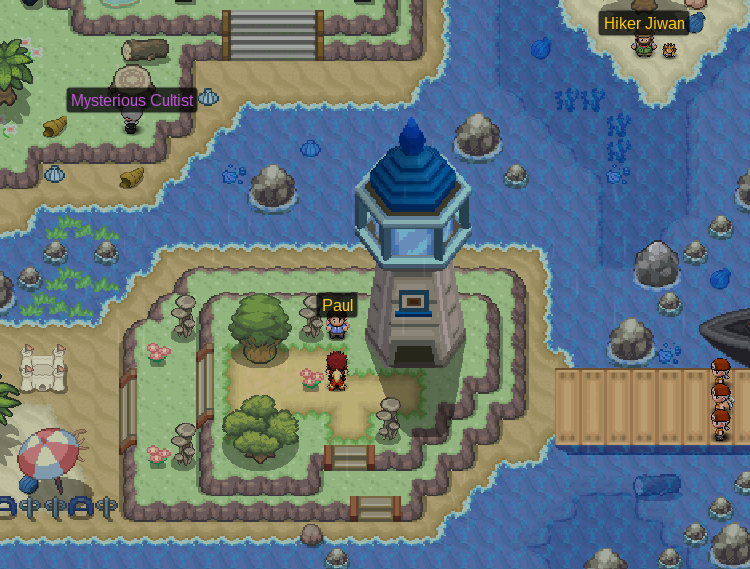
\includegraphics[width=\textwidth]{walkthrough/Sinnoh/paul-lilycove}

\subsection{In the Beginning}\label{subsec:in-the-beginning}

\subsubsection{Twinleaf Town}\label{subsubsec:twinleaf-town}
Welcome to Sinnoh.
Go downstairs and talk with your grandma.

\subsubsection{Route 201}\label{subsubsec:route_201}
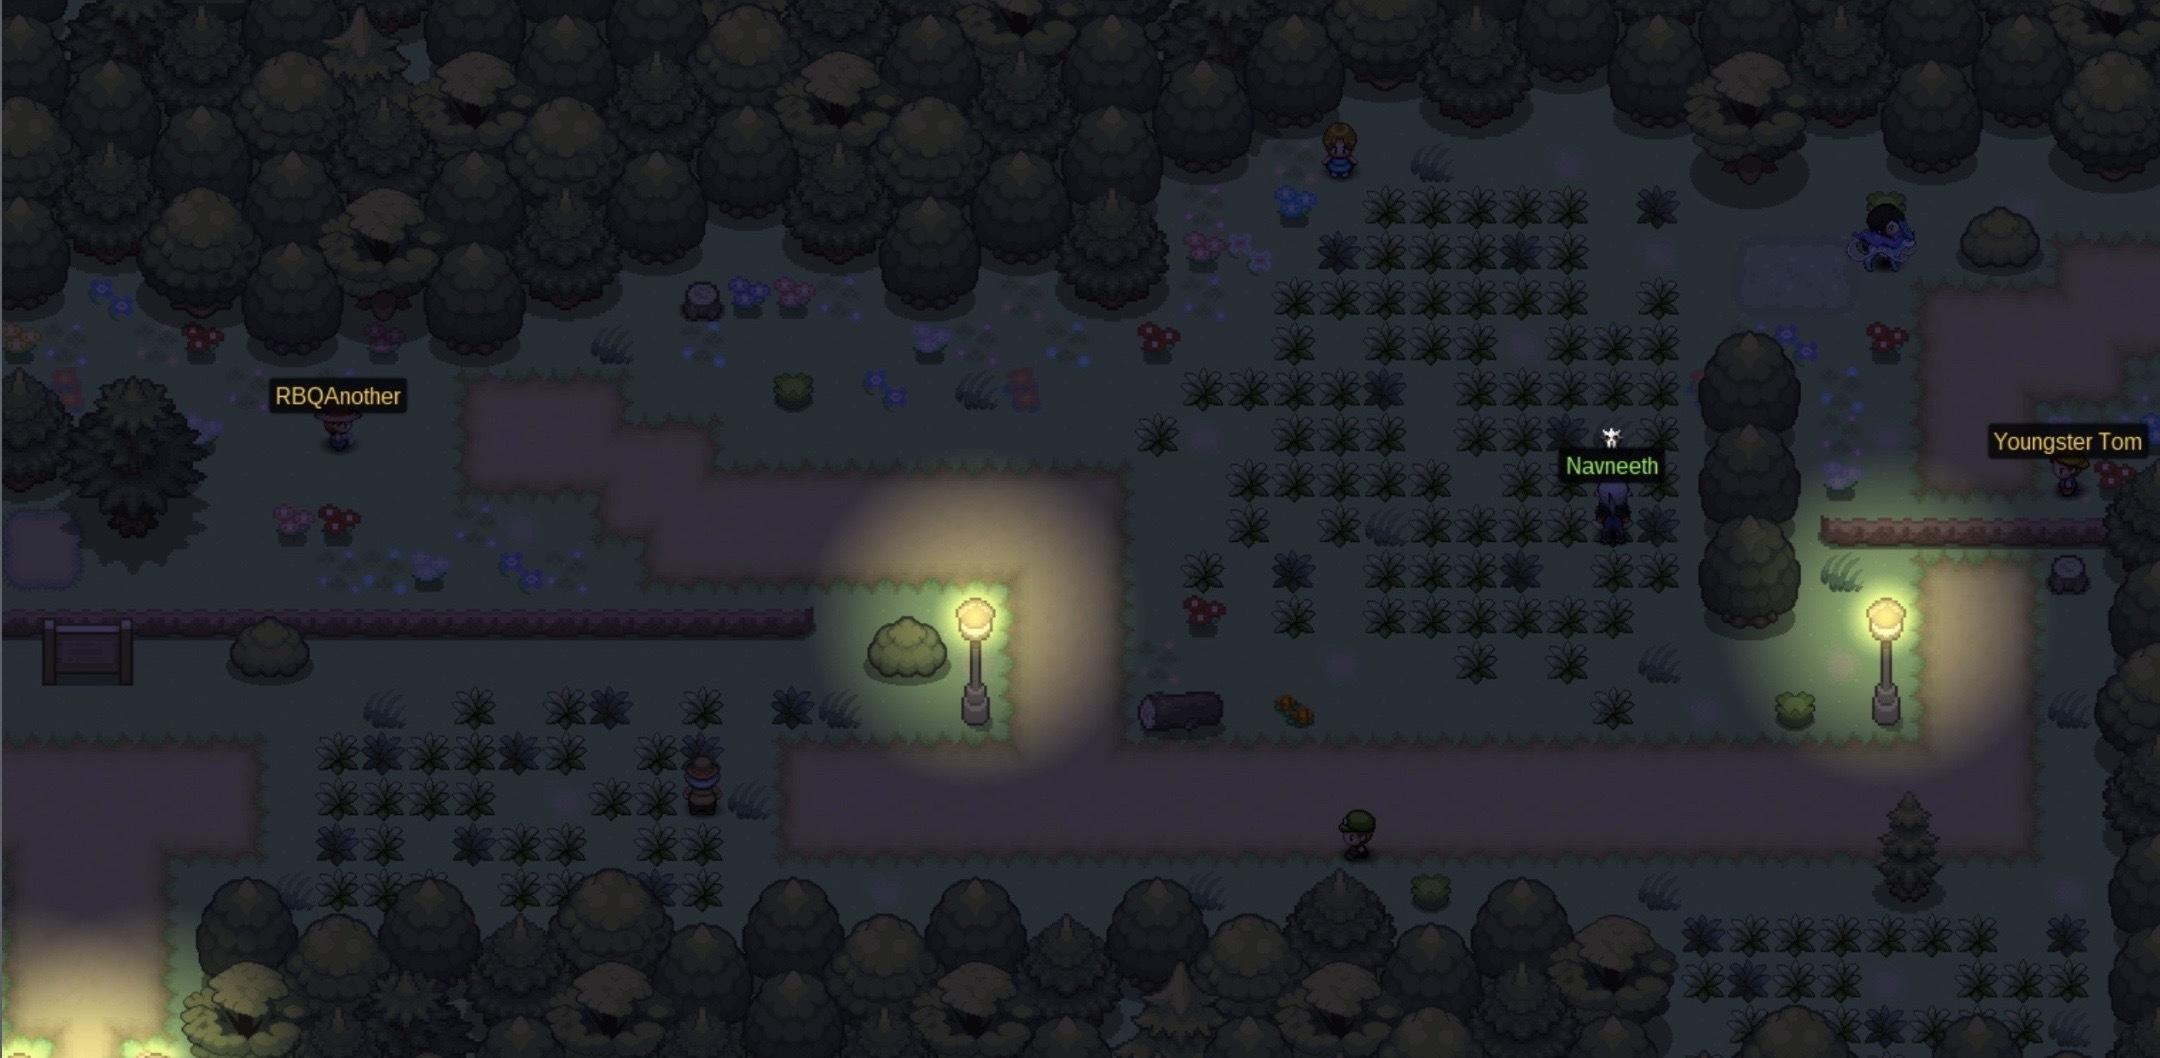
\includegraphics[width=\textwidth]{walkthrough/Sinnoh/Route_201}

Now we can go and visit Barry in his home, go up and talk with him
and then we can meet him in Route 201.
Prof  Rowan is going to stop us from walking in the grass without pokemon
and be ready to choose your starter.
Now go to the right and go to Prof Rowan lab.

\input{routes/Sinnoh/Route_201/Wild_Pokémon_(Land)}

\begin{mdframed}[style=PokemonSpotlight,nobreak=true,frametitle={Pokemon Spotlight: Bidoof}]
The humble Bidoof may not seem like an opposing foe, but some of them are \emph{Moody}.
The Hidden Ability \emph{Moody} raises one of the stats of the Pokémon with this
Ability by two stages (at random), then decreases another stat by one stage (at random).
A Bidoof or Bibarel that stays in battle long enough can reach maxed out stats
and become an unstoppable threat.

\begin{wrapfigure}{l}{0.33\textwidth}
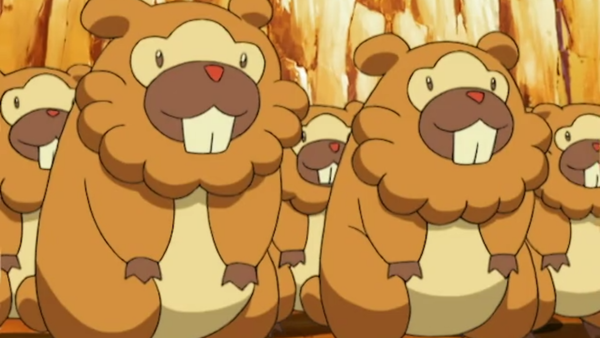
\includegraphics[width=0.33\textwidth]{walkthrough/Sinnoh/spotlight-bidoof}
\label{fig:spotlight-bidoof}
\end{wrapfigure}

The \emph{Moody} ability is perceived as so overpowered that Moody Bibarel has been
banned from most PvP formats.
Although \emph{Moody} will show up in only 5\% of Bidoofs, it may be worth the
grind in the early game to find one with this powerful ability, especially if
you do not pick Piplup as your starter.
The more common ability \emph{Simple} can also be utilized to double the effect of
\emph{Swords Dance} and make Bidoof/Bibarel a threatening foe.
Look for one with an Adamant nature and high IVs in Attack and Speed.
\end{mdframed}

\subsubsection{Lake Verity}\label{subsubsec:lake_verity}

\input{routes/Sinnoh/Lake_Verity/Wild_Pokémon_(Land)}
\input{routes/Sinnoh/Lake_Verity/Wild_Pokémon_(Water)}

\subsubsection{Sandgem Town}\label{subsubsec:sandgem-town}
Go to the Lab and we will find Barry.
He will tell us that he is going to be at Jubilife School.
Enter the Lab and talk with Prof Rowan, But we already have everything from Prof Oak.

\subsubsection{Back to Grandma}\label{subsubsec:back-to-grandma}
After talking with Prof Rowan we cant go to Route 202.
First we need to talk with our Grandma.
Go back to your house and talk with Grandma.
She will tell us that Barry's mom is worried, We need to visit her too.
Talk with his mother and she is going to ask us to tell Barry to go back home, he forgot something.

\subsection{Jubilife Gym}\label{subsec:jubilife-gym}

\subsubsection{Route 202}\label{subsubsec:route_202}
After talking with Grandma and Barry's mom, we can move on to Route 202.

\input{routes/Sinnoh/Route_202/Wild_Pokémon_(Land)}
\begin{longtable}{|| l l l l ||}%
\hline%
&Potion&x 2{-}3&Not respawnable\\%
\multicolumn{4}{||m{\textwidth}||}{In the middle of the south-westmost patch of grass.}%
\hline%
&Pokeball&x 5&Not respawnable\\%
\multicolumn{4}{||m{\textwidth}||}{Partially hidden by a tree at the north-westmost patch of grass.}%
\hline%
\endhead%
\hline%
\caption{Items in Route 202}%
\label{tab:Route202Items}%
\end{longtable}

\subsubsection{Jubilife City}\label{subsubsec:jubilife-city}
Once in Jubilife city we need to find barry in the school.

\paragraph{Student Locations}\label{par:student-locations}
Unfortunately, Barry is not there and we will have to help the teacher find her students first.

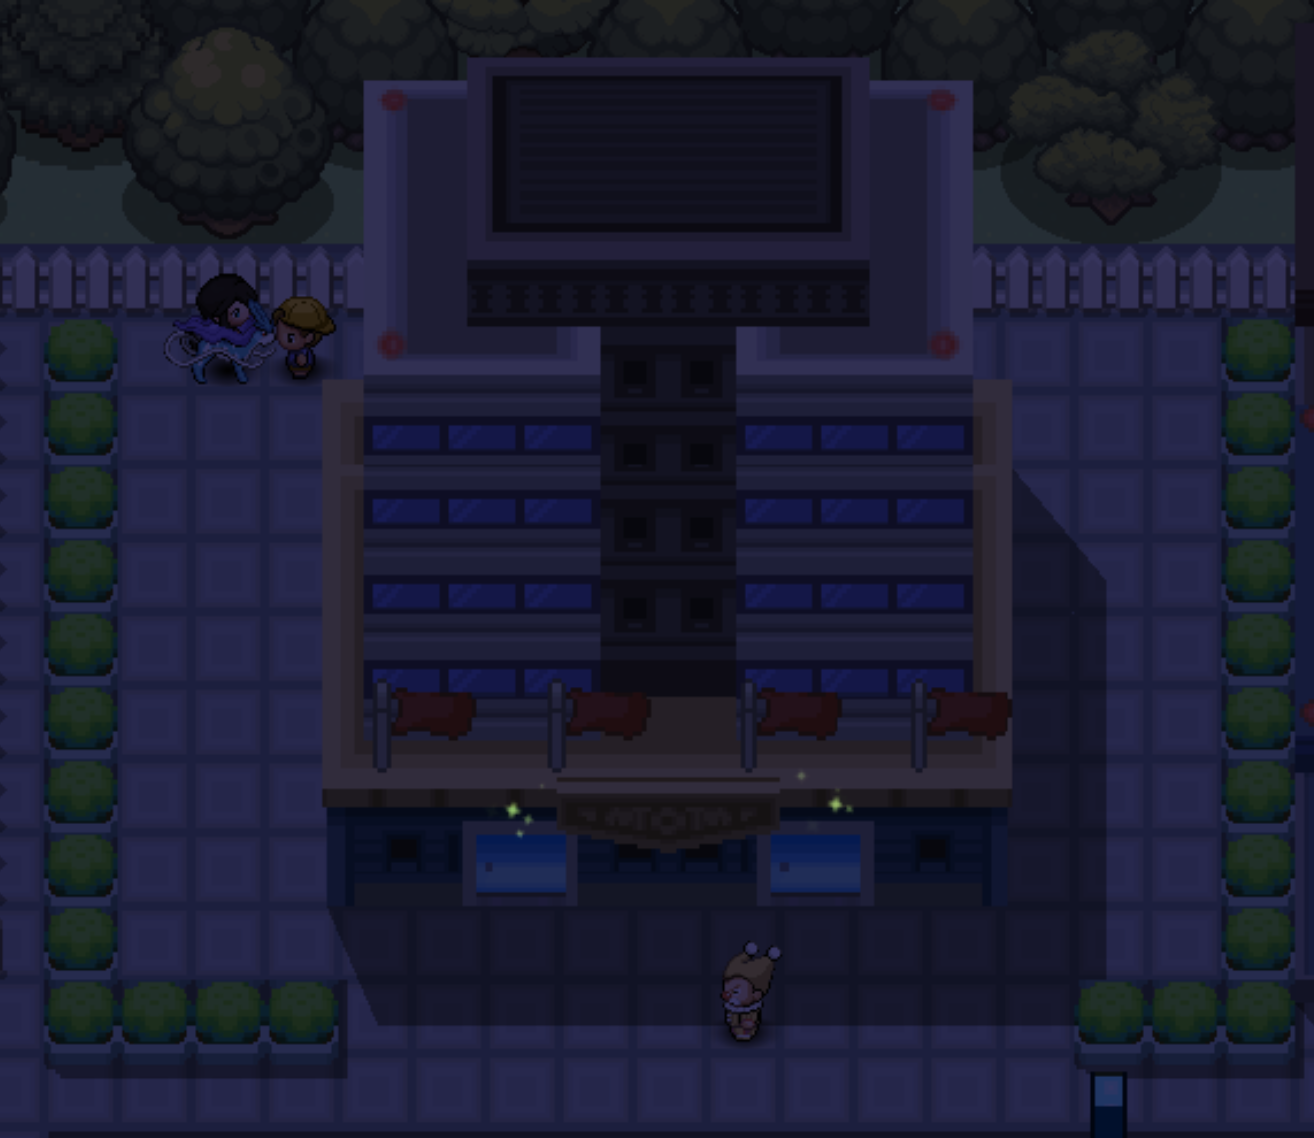
\includegraphics[width=0.5\textwidth]{walkthrough/Sinnoh/Jubilife-student-1}
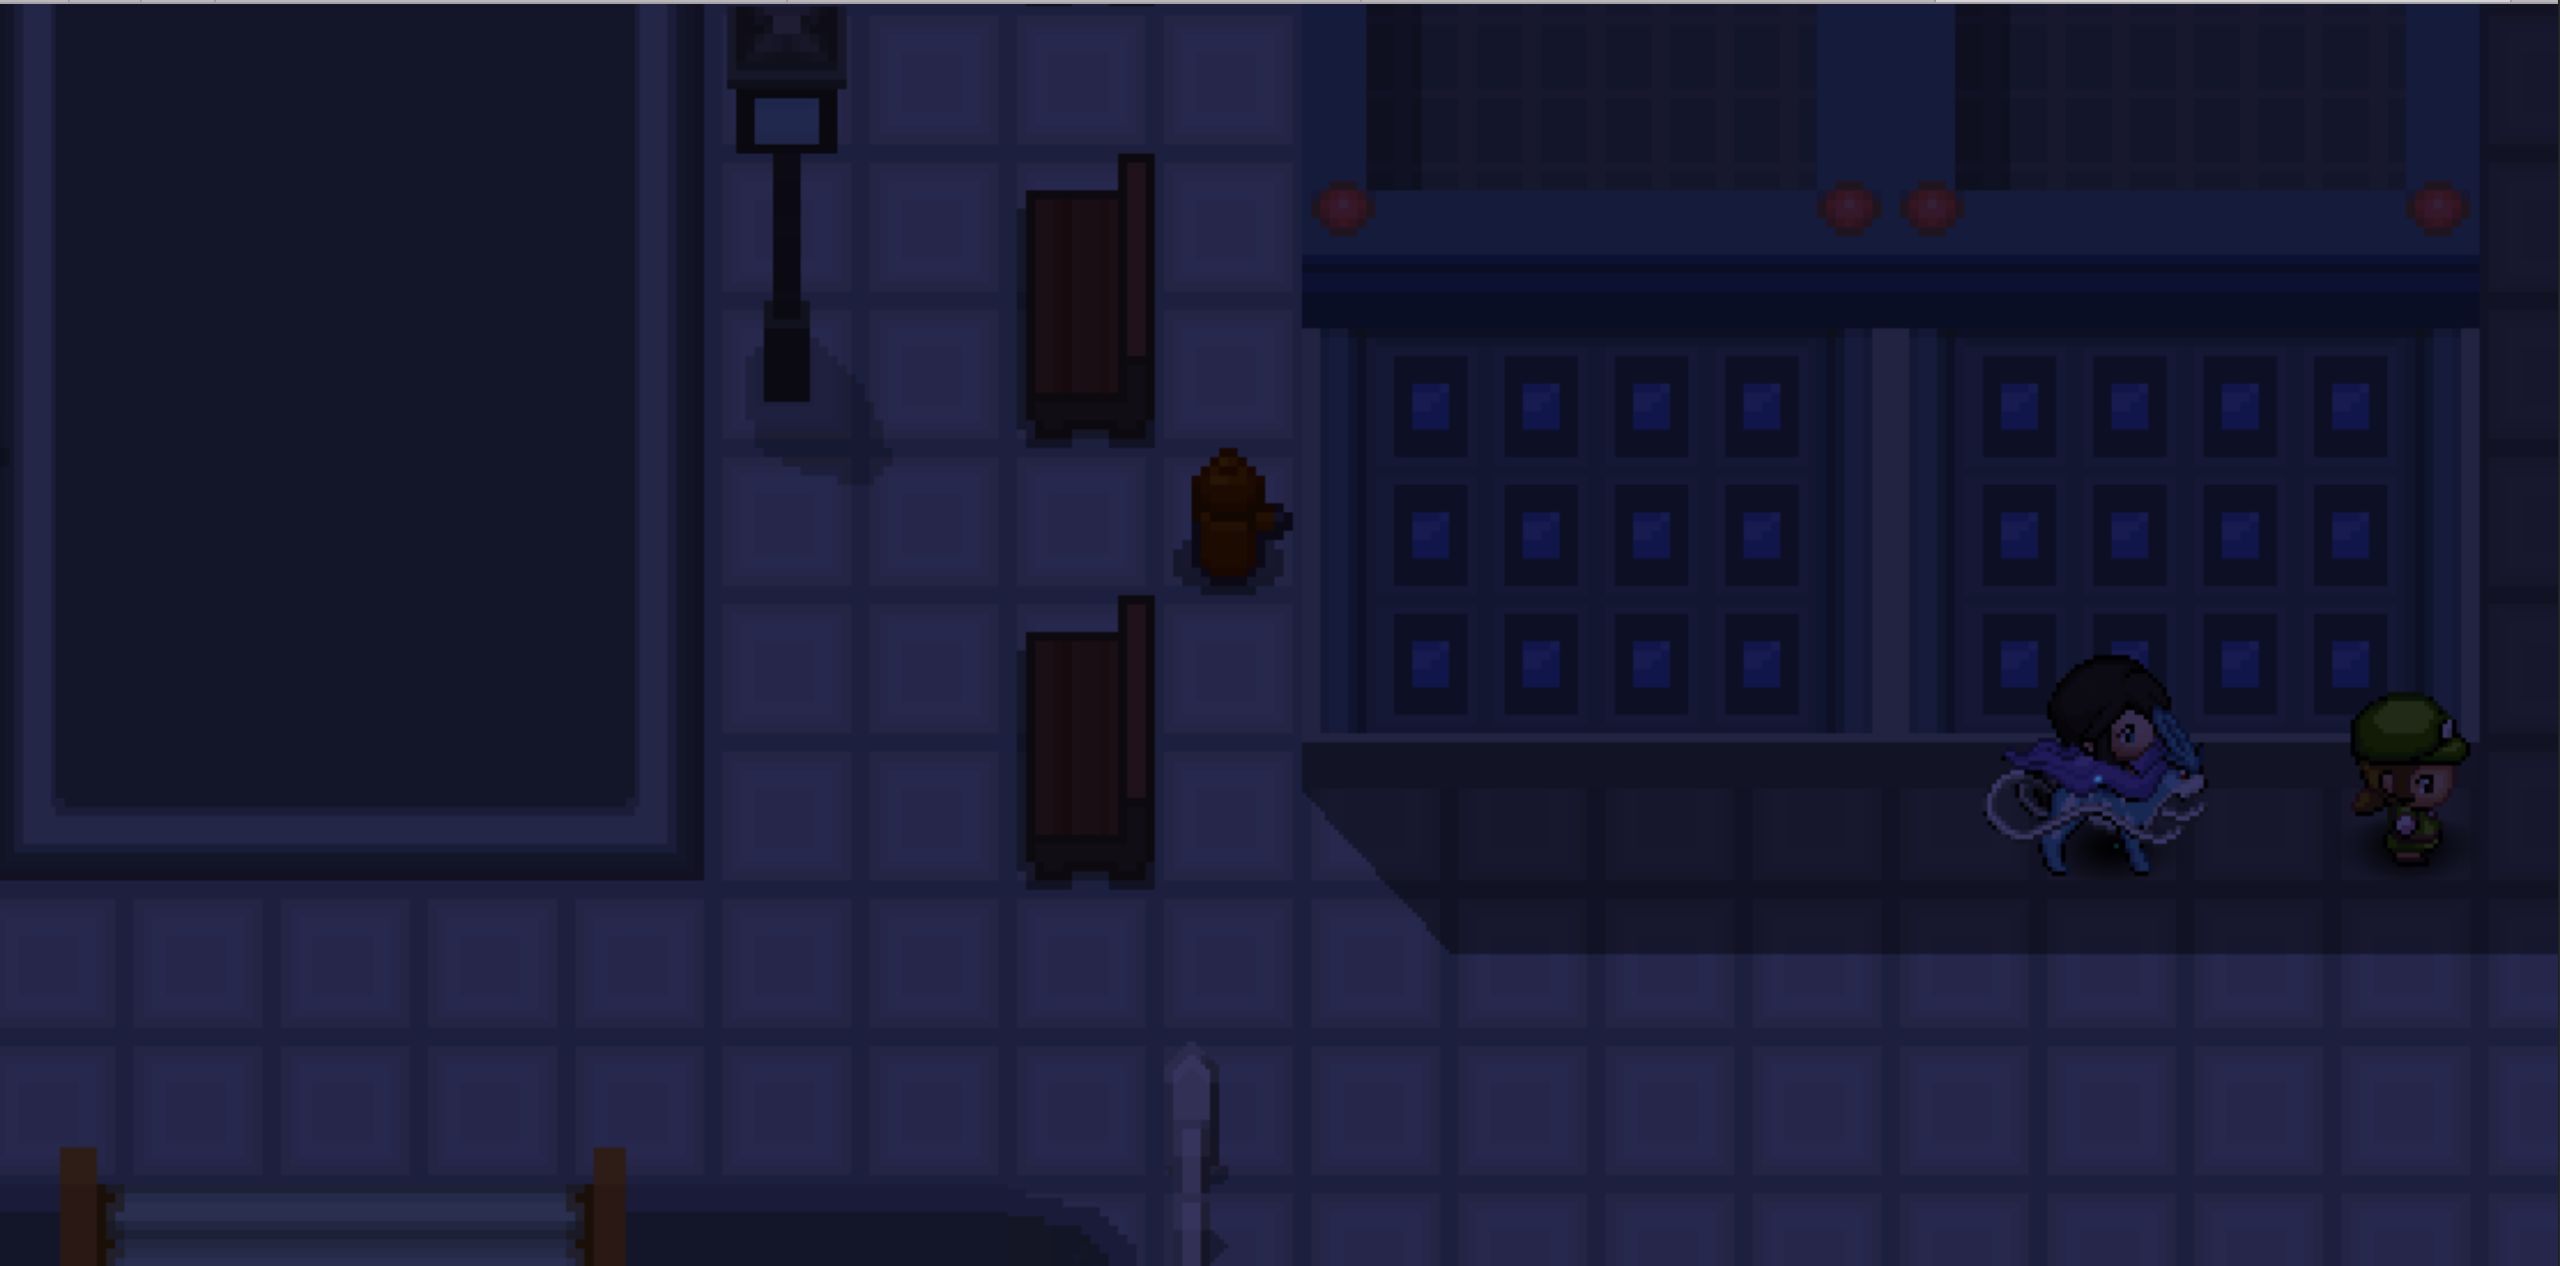
\includegraphics[width=0.5\textwidth]{walkthrough/Sinnoh/Jubilife-student-2}
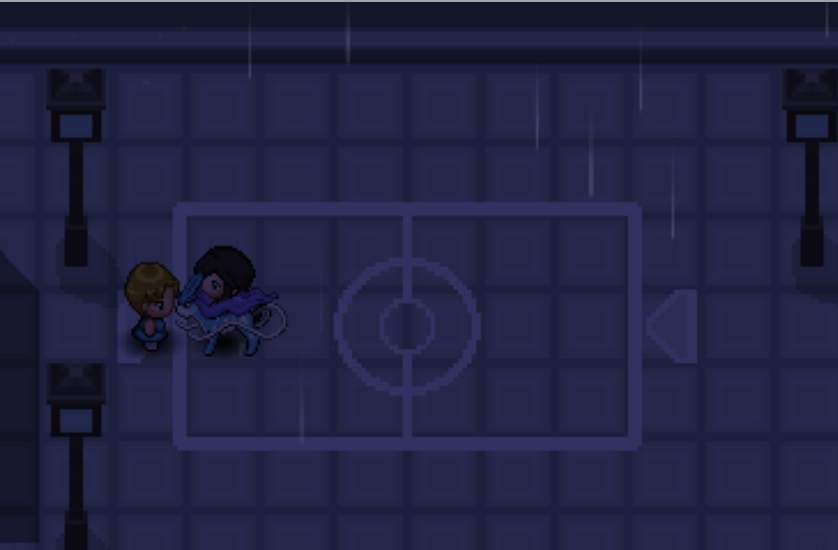
\includegraphics[width=0.5\textwidth]{walkthrough/Sinnoh/Jubilife-student-3}
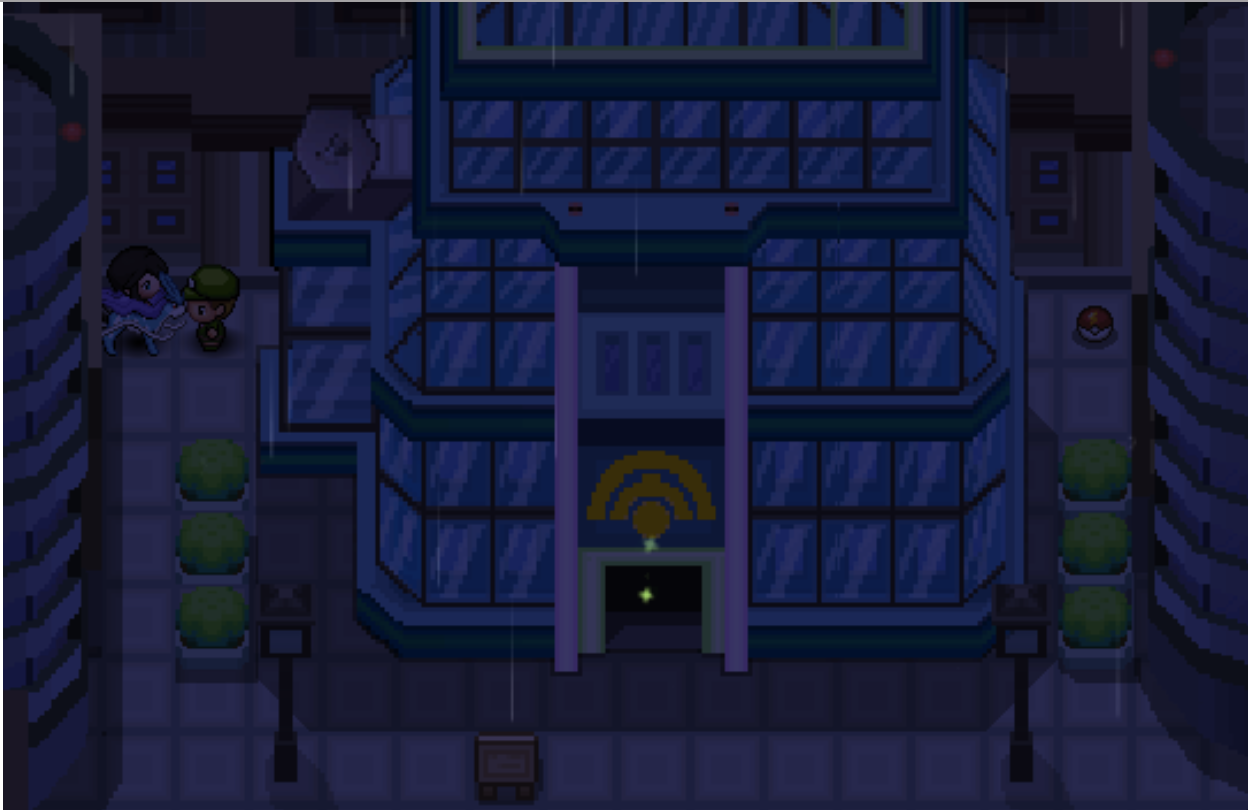
\includegraphics[width=0.5\textwidth]{walkthrough/Sinnoh/Jubilife-student-4}

And then go back to the school and talk with the Teacher.

\subsubsection{Route 218}\label{subsubsec:route_218}
Now we can find Barry at Route 218.
He will go back to his house and then we can go to Route 203.

\input{routes/Sinnoh/Route_218/Wild_Pokémon_(Land)}
\begin{longtable}{|| l l l l ||}%
\hline%
&Rare Candy&x 1&Not respawnable\\%
\multicolumn{4}{||m{\textwidth}||}{In the north-east corner of the route. Requires Surf.}%
\hline%
&Cheri Berry&x 1{-}3&3 days\\%
\multicolumn{4}{||m{\textwidth}||}{In the north-east of the patch of grass.}%
\hline%
&Qualot Berry&x 1{-}4&4 days\\%
\multicolumn{4}{||m{\textwidth}||}{In the north-east of the patch of grass.}%
\hline%
&Grepa Berry&x 1{-}4&4 days\\%
\multicolumn{4}{||m{\textwidth}||}{In the north-east of the patch of grass.}%
\hline%
\endhead%
\hline%
\caption{Items in Route 218}%
\label{tab:Route218Items}%
\end{longtable}

\subsubsection{Route 203}\label{subsubsec:route_203}
Be ready to battle with Barry.
Beat him and enter the cave in the right.

\input{routes/Sinnoh/Route_203/Wild_Pokémon_(Land)}
\input{routes/Sinnoh/Route_203/Wild_Pokémon_(Water)}
\begin{longtable}{|| l l l l ||}%
\hline%
&Great Ball&1{-}2&Not respawnable\\%
\hline%
&Repel&2&Not respawnable\\%
\hline%
\endhead%
\hline%
\caption{Items in Route 203}%
\label{tab:Route203Items}%
\end{longtable}

\subsubsection{Oreburgh Gate}\label{subsubsec:oreburgh-gate}
Ignore the upper route for now and go to the right.

\input{routes/Sinnoh/Oreburgh_Gate/Wild_Pokémon_(Oreburgh_Gate_1F)}
\begin{longtable}{|| l l l l ||}%
\hline%
&Moon Stone&1&3 days\\%
\hline%
&HP Up&1&3 days\\%
\hline%
&Stardust&1&3 days\\%
\hline%
&Rare Candy&1&3 days\\%
\hline%
&Protector&1&3 days\\%
\hline%
\endhead%
\hline%
\caption{Items in Oreburgh Gate}%
\label{tab:OreburghGateItems}%
\end{longtable}

\subsubsection{Oreburgh City}\label{subsubsec:oreburgh-city}
Now we are in the first city with a gym.
But first we need to Find Roark in the mine.

\subsection{Oreburgh Gym}\label{subsec:oreburgh-gym}

\subsubsection{Oreburgh Mine}\label{subsubsec:oreburgh-mine}

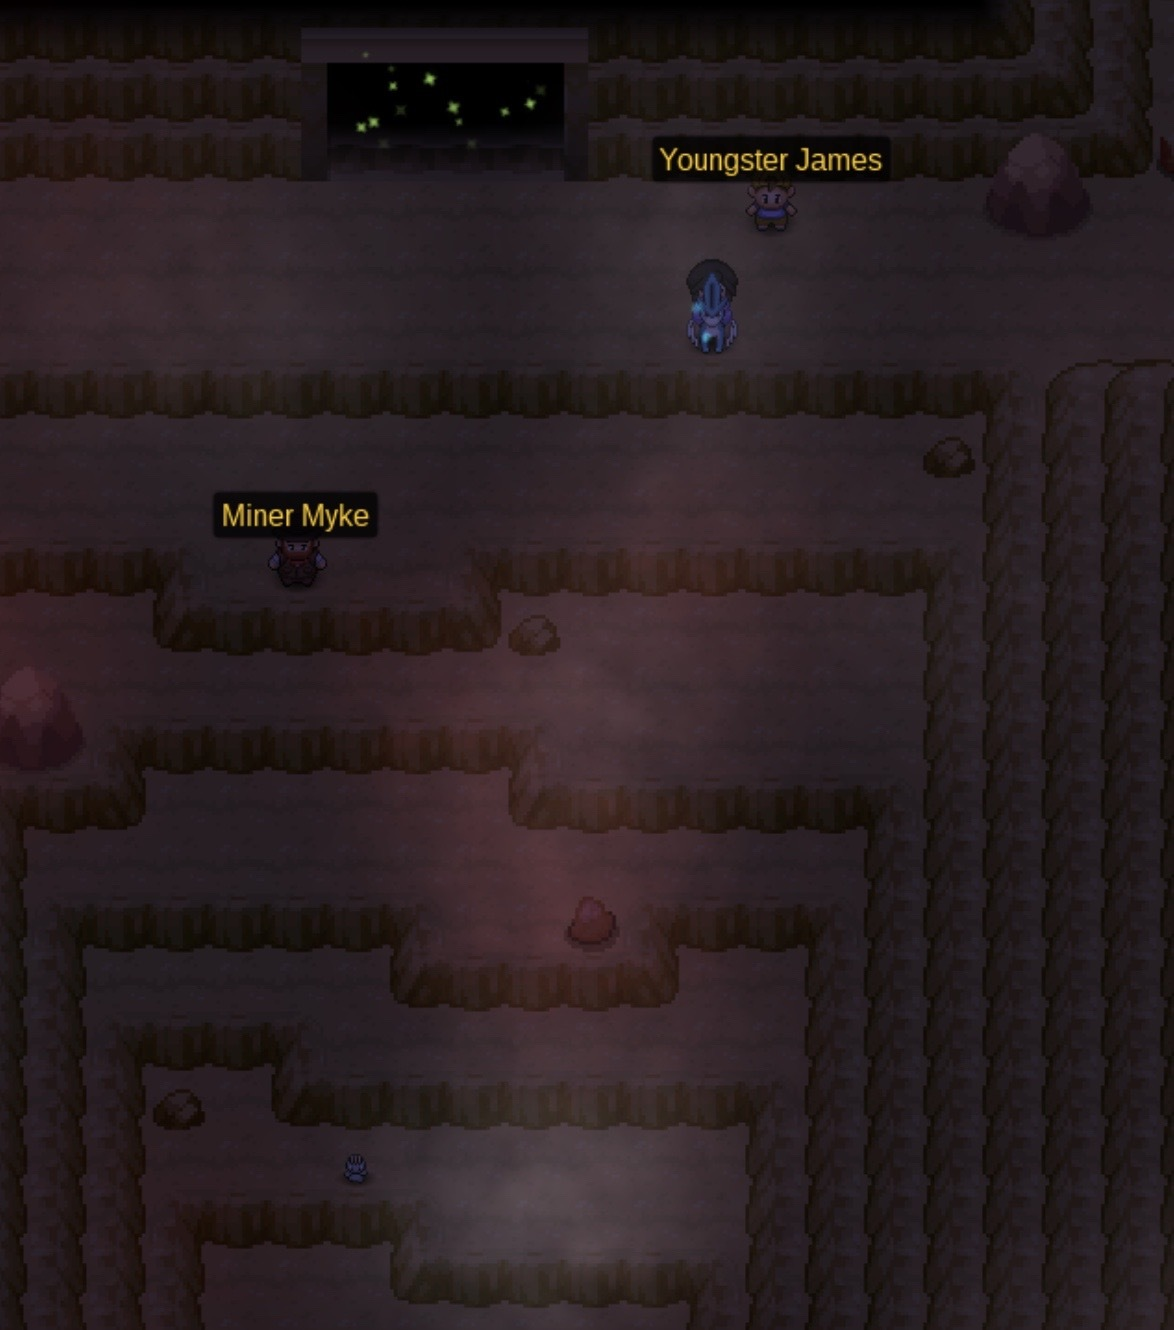
\includegraphics[width=\textwidth]{walkthrough/Sinnoh/oreburgh_mine}

Go all the way down to the mine and we are going to find him there,
talk with him and go back to the gym.

\input{routes/Sinnoh/Oreburgh_Mine/Wild_Pokémon_(Oreburgh_Mine_B1F)}
\input{routes/Sinnoh/Oreburgh_Mine/Wild_Pokémon_(Oreburgh_Mine_B2F_1R)}

\subsubsection{Oreburgh Gym}\label{subsubsec:oreburgh-gym}
Roark uses Rock-type pokemon.
After beating the gym go to Oreburgh City House 2 and you will find this NPC
selling rock smash, buy one we are going to need it later.

\subsubsection{Route 204}\label{subsubsec:route_204}
First head back to Jubilife City and talk with Looker and help him.
Now go to Route 204 and talk with the man in front of the cave enterence
in order to enter to the cave.

\input{routes/Sinnoh/Route_204/Wild_Pokémon_(Land)}
\input{routes/Sinnoh/Route_204/Wild_Pokémon_(Water)}
\begin{longtable}{|| l l l l ||}%
\hline%
&Paralyze Heal&x 1&Not respawnable\\%
\multicolumn{4}{||m{\textwidth}||}{At the end of the path beyond the east fence near the southern exit. The path can be entered from south of the fence.}%
\hline%
&HP Up&x 1&Not respawnable\\%
\multicolumn{4}{||m{\textwidth}||}{Hidden Item. Behind a tree at the end of the small path east of the north-east body of water.}%
\hline%
\endhead%
\hline%
\caption{Items in Route 204}%
\label{tab:Route204Items}%
\end{longtable}

\subsubsection{Ravaged Path}\label{subsubsec:ravaged_path2}
This is why we needed to buy rock smash, smash the rock and go to the next area.

\input{routes/Sinnoh/Ravaged_Path/Wild_Pokémon_(Land)}
\input{routes/Sinnoh/Ravaged_Path/Wild_Pokémon_(Water)}
\begin{longtable}{|| l l l l ||}%
\hline%
&Potion&1&3 days\\%
\hline%
&Dusk Stone&1&3 days\\%
\hline%
&Revive&1&3 days\\%
\hline%
&Big Pearl&1&3 days\\%
\hline%
&Macho Brace&1&3 days\\%
\hline%
\endhead%
\hline%
\caption{Items in Ravaged Path}%
\label{tab:RavagedPathItems}%
\end{longtable}

\subsection{Floaroma Town and Eterna Forest}\label{subsec:floaroma-town-and-eterna-forest}

\subsubsection{Valley Windworks}\label{subsubsec:valley-windworks}
Finally we are in Floaroma town but skip that town and go to route 205,
we are going to meet Sandy and we need to help her dad.
Go to the right and we are going to find Galactic Team again, Beat him.
Now we need a password to enter, Go back to Floaroma Town.

\input{routes/Sinnoh/Valley_Windworks/Wild_Pokémon_(Land)}
\input{routes/Sinnoh/Valley_Windworks/Wild_Pokémon_(Water)}
\begin{longtable}{|| l l l l ||}%
\hline%
&TM24 — Thunderbolt&x 1&Not respawnable\\%
\multicolumn{4}{||m{\textwidth}||}{Just over the fence west of the building. Requires Surf.}%
\hline%
&Super Potion&x 1&Not respawnable\\%
\multicolumn{4}{||m{\textwidth}||}{Hidden item. On the windmill directly in front of the building.}%
\hline%
\endhead%
\hline%
\caption{Items in Valley Windworks}%
\label{tab:ValleyWindworksItems}%
\end{longtable}

\subsubsection{Floaroma Town}\label{subsubsec:floaroma-town}
Back in Floaroma Town, go to the top left area.
Beat the galactic guy and he is going to give us the password.
Go back to Valley Windworks and get ready to battle.

\subsubsection{Route 205}\label{subsubsec:route_205}
After you beat galactic guy, Go back to Route 205 and go to the north.
Nothing important in this route just a lot of trainers to get a lot of XP,
Go to the top and enter to Eterna Forest.

\input{routes/Sinnoh/Route_205/Wild_Pokémon_(Land)}
\input{routes/Sinnoh/Route_205/Wild_Pokémon_(Water)}
\begin{longtable}{|| l l l l ||}%
\hline%
&Antidote&x 1&Not respawnable\\%
\multicolumn{4}{||m{\textwidth}||}{On the side of the mountain, just before the bridge connecting two mountain parts. Must be accessed by going down the grassy path.}%
\hline%
&TM138 — Sleep Talk&x 1&Not respawnable\\%
\multicolumn{4}{||m{\textwidth}||}{In the shortcut to skip Eterna Forest. Requires Cut.}%
\hline%
&Lum Berry&x 1{-}3&3 days\\%
\multicolumn{4}{||m{\textwidth}||}{Berry tree next to the Floaroma Town entrance.}%
\hline%
&Sitrus Berry&x 1{-}3&3 days\\%
\multicolumn{4}{||m{\textwidth}||}{Berry tree next to the Floaroma Town entrance.}%
\hline%
\endhead%
\hline%
\caption{Items in Route 205}%
\label{tab:Route205Items}%
\end{longtable}

\subsubsection{Eterna Forest}\label{subsubsec:eterna_forest}
Eterna forest have a lot of trainers as well.
After you beat them all go to the top right and you are in the second area of route 205.

\input{routes/Sinnoh/Eterna_Forest/Wild_Pokémon_(Land)}
\input{routes/Sinnoh/Eterna_Forest/Wild_Pokémon_(Headbuttable_Trees)}
\begin{longtable}{|| l l l l ||}%
\hline%
&Antidote&x 1&Not respawnable\\%
\multicolumn{4}{||m{\textwidth}||}{On the upper far west side of the forest.}%
\hline%
&Paralyze Heal&x 2&Not respawnable\\%
\multicolumn{4}{||m{\textwidth}||}{In the south-east part, along the eastmost path.}%
\hline%
&Great Ball&x 2&Not respawnable\\%
\multicolumn{4}{||m{\textwidth}||}{In the far north, next to the Old Chateau. Requires Cut.}%
\hline%
&Insect Plate&x 1&Not respawnable\\%
\multicolumn{4}{||m{\textwidth}||}{Hidden item. On the plant immediately to the east of the Old Chateau. Requires Cut.}%
\hline%
\endhead%
\hline%
\caption{Items in Eterna Forest}%
\label{tab:EternaForestItems}%
\end{longtable}

\subsection{Eterna Gym and Galactic Eterna Building}\label{subsec:eterna-gym}

\subsubsection{Eterna City}\label{subsubsec:eterna-city}
Now we are in Eterna City.
Go to the gym and you are going to find Gardenia outside and she will ask you
if you can check the building in the north of the city.
Go to the building and we are going to find grunts for Galactic Team again.
Be ready to battle.
Once in the building go to the top and you will find
Commander Jupiter and Jevons, Talk with Jupiter and beat him.
After you beat him talk with Devons and help him to find some pokemon.
Pokemon Locations: TBD

After you find all pokemons, Talk with Jevons again and then go to the gym.

\subsubsection{Eterna City Gym}\label{subsubsec:eterna-city-gym}
Gardenia uses Grass-type Pokemon.
Beat her and get the badge.

\subsubsection{Route 211 (West)}\label{subsubsec:route_211_(west)}

\input{routes/Sinnoh/Route_211/Wild_Pokémon_(Land)}

\subsubsection{Mt. Coronet (Northern Area Part 1)}\label{subsubsec:mt._coronet_north}
% \subsubsection{Wild Pokémon (Mt. Coronet North)}%
\label{ssubsec:WildPokmon(Mt.CoronetNorth)}%
\begin{longtable}{||l l l l l l l l||}%
\hline%
\rowcolor{gray}%
&Pokémon&Level Range&Morn&Day&Night&Held Item&Rarity Tier\\%
\hline%
\endhead%
\hline%
\rowcolor{gray}%

\includegraphics[width=0.02\textwidth]{pokemon/Cleffa}&Cleffa&13{-}17&Morn&Day&Night&Leppa Berry&\textcolor{RedOrange}{%
Rare%
}\\%
\hline%
\rowcolor{gray}%

\includegraphics[width=0.02\textwidth]{pokemon/Geodude}&Geodude&13{-}17&Morn&Day&Night&&\textcolor{black}{%
Common%
}\\%
\hline%
\rowcolor{gray}%

\includegraphics[width=0.02\textwidth]{pokemon/Gible}&Gible&5{-}14&Morn&&Night&&\textcolor{RedOrange}{%
Rare%
}\\%
\hline%
\rowcolor{gray}%

\includegraphics[width=0.02\textwidth]{pokemon/Machop}&Machop&13{-}17&Morn&Day&Night&&\textcolor{black}{%
Common%
}\\%
\hline%
\rowcolor{gray}%

\includegraphics[width=0.02\textwidth]{pokemon/Zubat}&Zubat&13{-}17&Morn&Day&Night&&\textcolor{black}{%
Common%
}\\%
\hline%
\end{longtable}%
\caption{Wild Pokemon in Mt. Coronet North (Mt. Coronet North)}

\subsubsection{Old Chateau}\label{subsubsec:old_chateau}

\input{routes/Sinnoh/Old_Chateau/Wild_Pokémon_(Old_Chateau_1F)}
\begin{longtable}{|| l l l l ||}%
\hline%
&Dread Plate&x 1&Indefinite\\%
\multicolumn{4}{||m{\textwidth}||}{In 2F 1R, the westmost room of 2F.}%
\hline%
\endhead%
\hline%
\caption{Items in Old Chateau}%
\label{tab:OldChateauItems}%
\end{longtable}

\subsection{Path to Hearthome City}\label{subsec:path-to-hearthome-city}

\subsubsection{Route 206}\label{subsubsec:route_206}
Nothing important in this routes just beat all the trainers to get Xp.

\subsubsection{Wayward Cave}\label{subsubsec:wayward_cave}

\input{routes/Sinnoh/Wayward_Cave/Wild_Pokémon_(Wayward_Cave)}

\subsubsection{Route 207}\label{subsubsec:route_207}
In the cave from route 207 you will find Cyrus but you are not going to have a battle.

\input{routes/Sinnoh/Route_207/Wild_Pokémon_(Land)}
\begin{longtable}{|| l l l l ||}%
\hline%
&Iron&1&Not respawnable\\%
\hline%
&Revival Herb&1&Not respawnable\\%
\hline%
&Revive&1&Not respawnable\\%
\hline%
&Oran Berry&1{-}3&3 days\\%
\hline%
&Cheri Berry&1{-}3&3 days\\%
\hline%
&Sitrus Berry&1{-}2&3 days\\%
\hline%
&Lum Berry&1{-}2&3 days\\%
\hline%
\endhead%
\hline%
\caption{Items in Route 207}%
\label{tab:Route207Items}%
\end{longtable}

\begin{mdframed}[style=MyFrame,nobreak=true,frametitle={Pokemon Spotlight: Gligar}]

\begin{wrapfigure}{l}{0.33\textwidth}
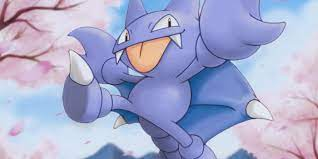
\includegraphics[width=0.33\textwidth]{walkthrough/Sinnoh/spotlight-gligar}
\label{fig:spotlight-gligar}
\end{wrapfigure}

Gligar's Hidden Ability, Poison Heal, allows it to be immune to status effects
when poisoned while also providing it with passive recovery, which is useful
alongside reliable recovery in Roost.
Using a Toxic Orb allows the poison to be applied automatically.

Gligar evolves into Gliscor when leveled up holding a Razor Fang during the night.
Find one with a Careful nature with high IVs in HP, Special Defense, and Speed.

If you don't want to grind for a Gligar with Poison Heal, a viable build can
also be made using Hyper Cutter.
Jolly or Impish Nature can also work.

\end{mdframed}

\subsubsection{Mt. Coronet South}\label{subsubsec:mt.-coronet-south}
TODO

\subsubsection{Route 208}\label{subsubsec:route_208}

\input{routes/Sinnoh/Route_208/Wild_Pokémon_(Land)}
\input{routes/Sinnoh/Route_208/Wild_Pokémon_(Water)}
\input{routes/Sinnoh/Route_208/Wild_Pokémon_(Headbuttable_Trees)}
\begin{longtable}{|| l l l l ||}%
\hline%
&Star Piece&1&Not respawnable\\%
\hline%
&Ultra Ball&2&Not respawnable\\%
\hline%
&Rawst Berry&1{-}2&3 days\\%
\hline%
&Pecha Berry&1{-}3&3 days\\%
\hline%
\endhead%
\hline%
\caption{Items in Route 208}%
\label{tab:Route208Items}%
\end{longtable}

\subsection{Hearthome City}\label{subsec:hearthome-city}

\subsubsection{Hearthome City}\label{subsubsec:hearthome-city}
Now we are in Hearthome but the Gym is not available to us yet.
Proceed along to the right and find Barry, Be ready to battle.

\paragraph{Notables}\label{par:notables-hearthome}

\begin{itemize}
    \item Caught Date Checker
    \item Move Relearner
    \item Move Tutor: Role Play
    \item TM Seller: Curse
\end{itemize}

\subsubsection{Amity Square}\label{subsubsec:amity-square}

\input{routes/Sinnoh/Amity_Square/Wild_Pokémon_(Land)}
\input{routes/Sinnoh/Amity_Square/Wild_Pokémon_(Water)}

\subsubsection{Route 209}\label{subsubsec:route_2092}

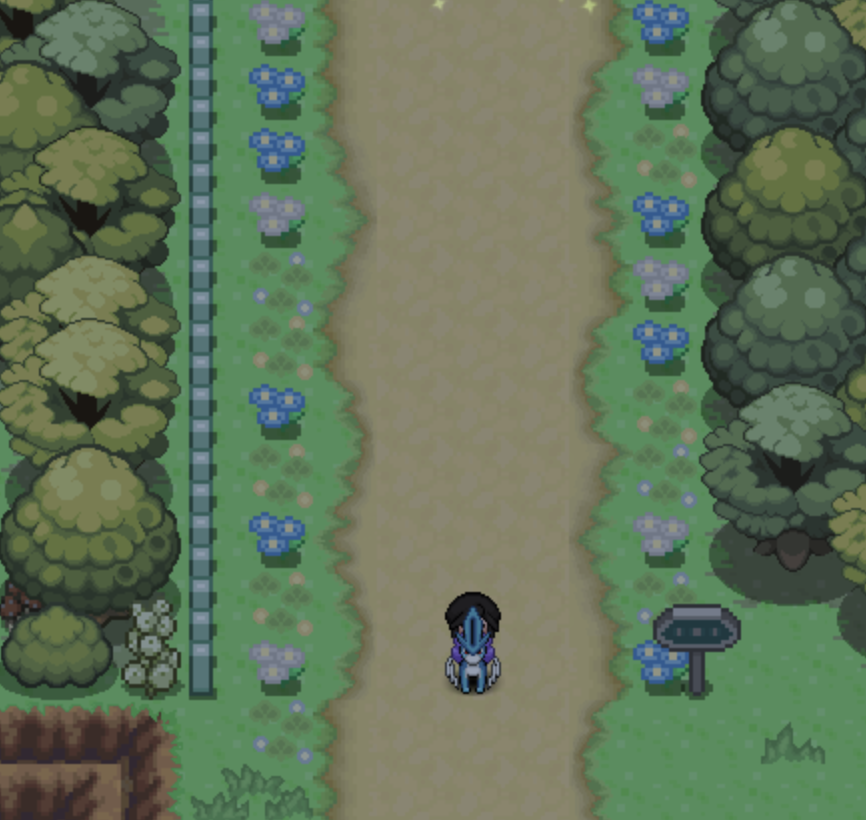
\includegraphics[width=\textwidth]{walkthrough/Sinnoh/Route_209}

Nothing important in this routes just battle with trainers

\input{routes/Sinnoh/Route_209/Wild_Pokémon_(Land)}
\input{routes/Sinnoh/Route_209/Wild_Pokémon_(Headbuttable_Trees)}
% \input{routes/Sinnoh/Route_209/Wild_Pokémon_(Diggable_Patches)}
\begin{longtable}{|| l l l l ||}%
\hline%
&Awakening&2&Not respawnable\\%
\hline%
&Hyper Potion&2&Not respawnable\\%
\hline%
&Elixir&1&Not respawnable\\%
\hline%
&Calcium&1&Not respawnable\\%
\hline%
&Lum Berry&1{-}2&3 days\\%
\hline%
&Leppa Berry&1{-}2&3 days\\%
\hline%
&Oran Berry&1{-}3&3 days\\%
\hline%
&Ultra Ball&1&3 days\\%
\hline%
&Protein&1&3 days\\%
\hline%
&PP Up&1&3 days\\%
\hline%
&Nugget&1&3 days\\%
\hline%
&Electirizer&1&3 days\\%
\hline%
\endhead%
\hline%
\caption{Items in Route 209}%
\label{tab:Route209Items}%
\end{longtable}

\begin{mdframed}[style=MyFrame,nobreak=true,frametitle={Pokemon Spotlight: Chansey}]

Chansey's augmented physical bulk with Eviolite allows it to take powerful physical hits,
making it a staple on defensively oriented teams.
Wish and Natural Cure allow Chansey to heal its teammates and absorb status for them,
while access to Seismic Toss and Toxic helps prevent it from being setup bait.

\begin{wrapfigure}{l}{0.33\textwidth}
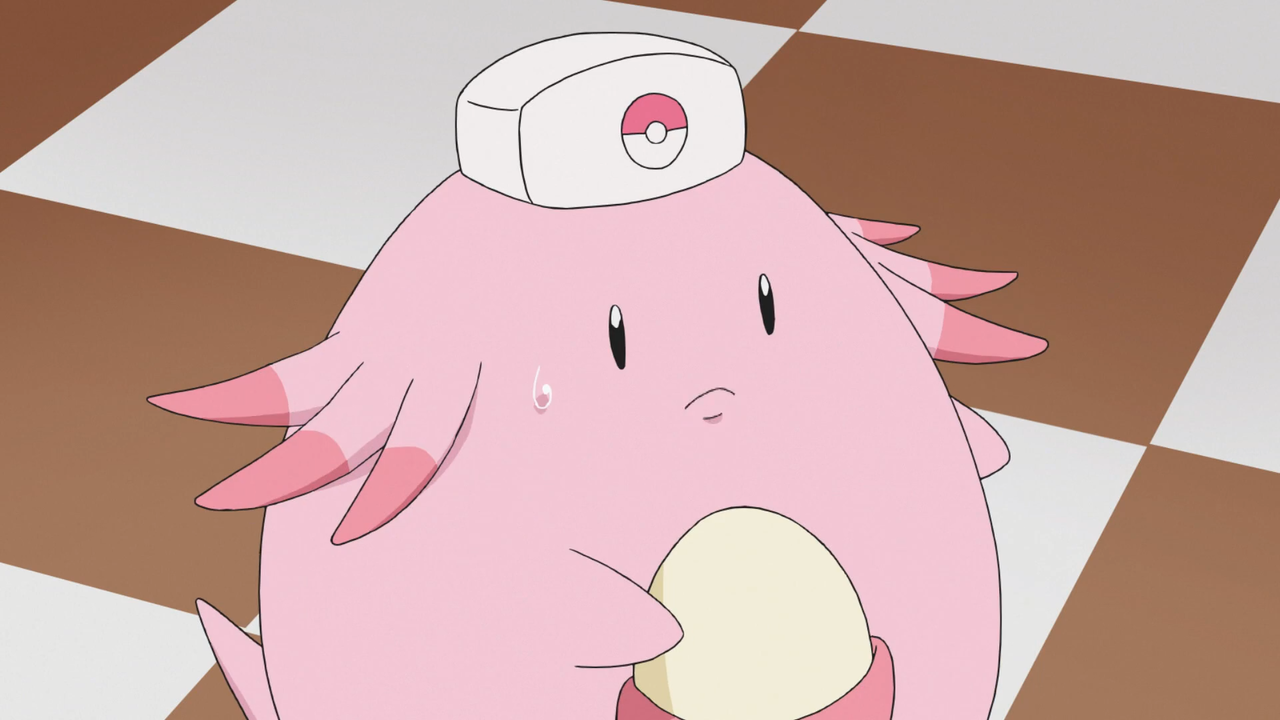
\includegraphics[width=0.33\textwidth]{walkthrough/Sinnoh/spotlight-chansey}
\label{fig:spotlight-chansey}
\end{wrapfigure}

Even with two ways of dealing damage, Chansey is still very passive and reliant on
Eviolite, and because of this it is largely shut down by Taunt or Knock Off.
Find one with a Bold nature with high IVs in Defense and Special Defense.

\end{mdframed}

\subsection{Solaceon Town}\label{subsec:solaceon-town}

\subsubsection{Lost Tower}\label{subsubsec:lost_tower}

Lost Tower is a Sinnoh tower located in the north of Route 209.
There isn’t anything interesting in the tower however,
making it a side area for catching Pokémons and getting a couple items.
At the top of the tower the nice lady will give you a \emph{Spell Tag}.

\input{routes/Sinnoh/Lost_Tower/Wild_Pokémon_(Lost_Tower_1F)}
\input{routes/Sinnoh/Lost_Tower/Wild_Pokémon_(Lost_Tower_2F)}
\input{routes/Sinnoh/Lost_Tower/Wild_Pokémon_(Lost_Tower_3F)}
\input{routes/Sinnoh/Lost_Tower/Wild_Pokémon_(Lost_Tower_4F)}
\begin{longtable}{|| l l l l ||}%
\hline%
&Oval Stone&1&Not respawnable\\%
\hline%
&Revive&1&Not respawnable\\%
\hline%
&Great Ball&3&Not respawnable\\%
\hline%
\endhead%
\hline%
\caption{Items in Lost Tower}%
\label{tab:LostTowerItems}%
\end{longtable}

\subsubsection{Route 210}\label{subsubsec:route_210}

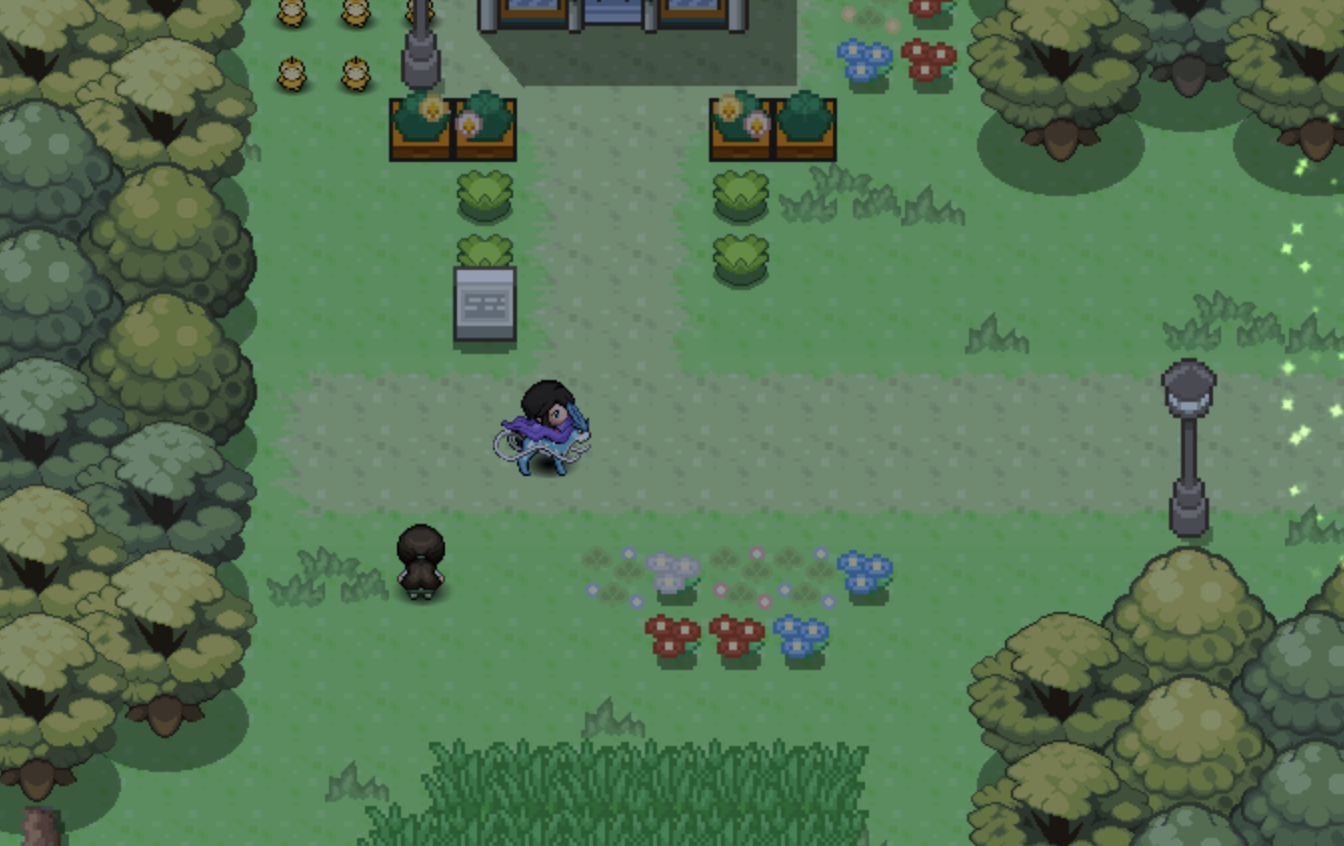
\includegraphics[width=\textwidth]{walkthrough/Sinnoh/Route_210}

\input{routes/Sinnoh/Route_210/Wild_Pokémon_(Land)}
\begin{longtable}{|| l l l l ||}%
\hline%
&Hyper Potion&2{-}4&Not respawnable\\%
\hline%
&Ultra Ball&2{-}4&Not respawnable\\%
\hline%
&Leppa Berry&1{-}2&3 days\\%
\hline%
&Lum Berry&1{-}2&3 days\\%
\hline%
\endhead%
\hline%
\caption{Items in Route 210}%
\label{tab:Route210Items}%
\end{longtable}

\subsubsection{Solaceon Town}\label{subsubsec:solaceon-town}

\paragraph{Notables}\label{par:notables-solaceon-town}

\begin{itemize}
    \item News Reporter
    \item Daycare
\end{itemize}

\subsection{Veilstone Gym}\label{subsec:veilstone-gym}

\subsubsection{Route 215}\label{subsubsec:route_215}

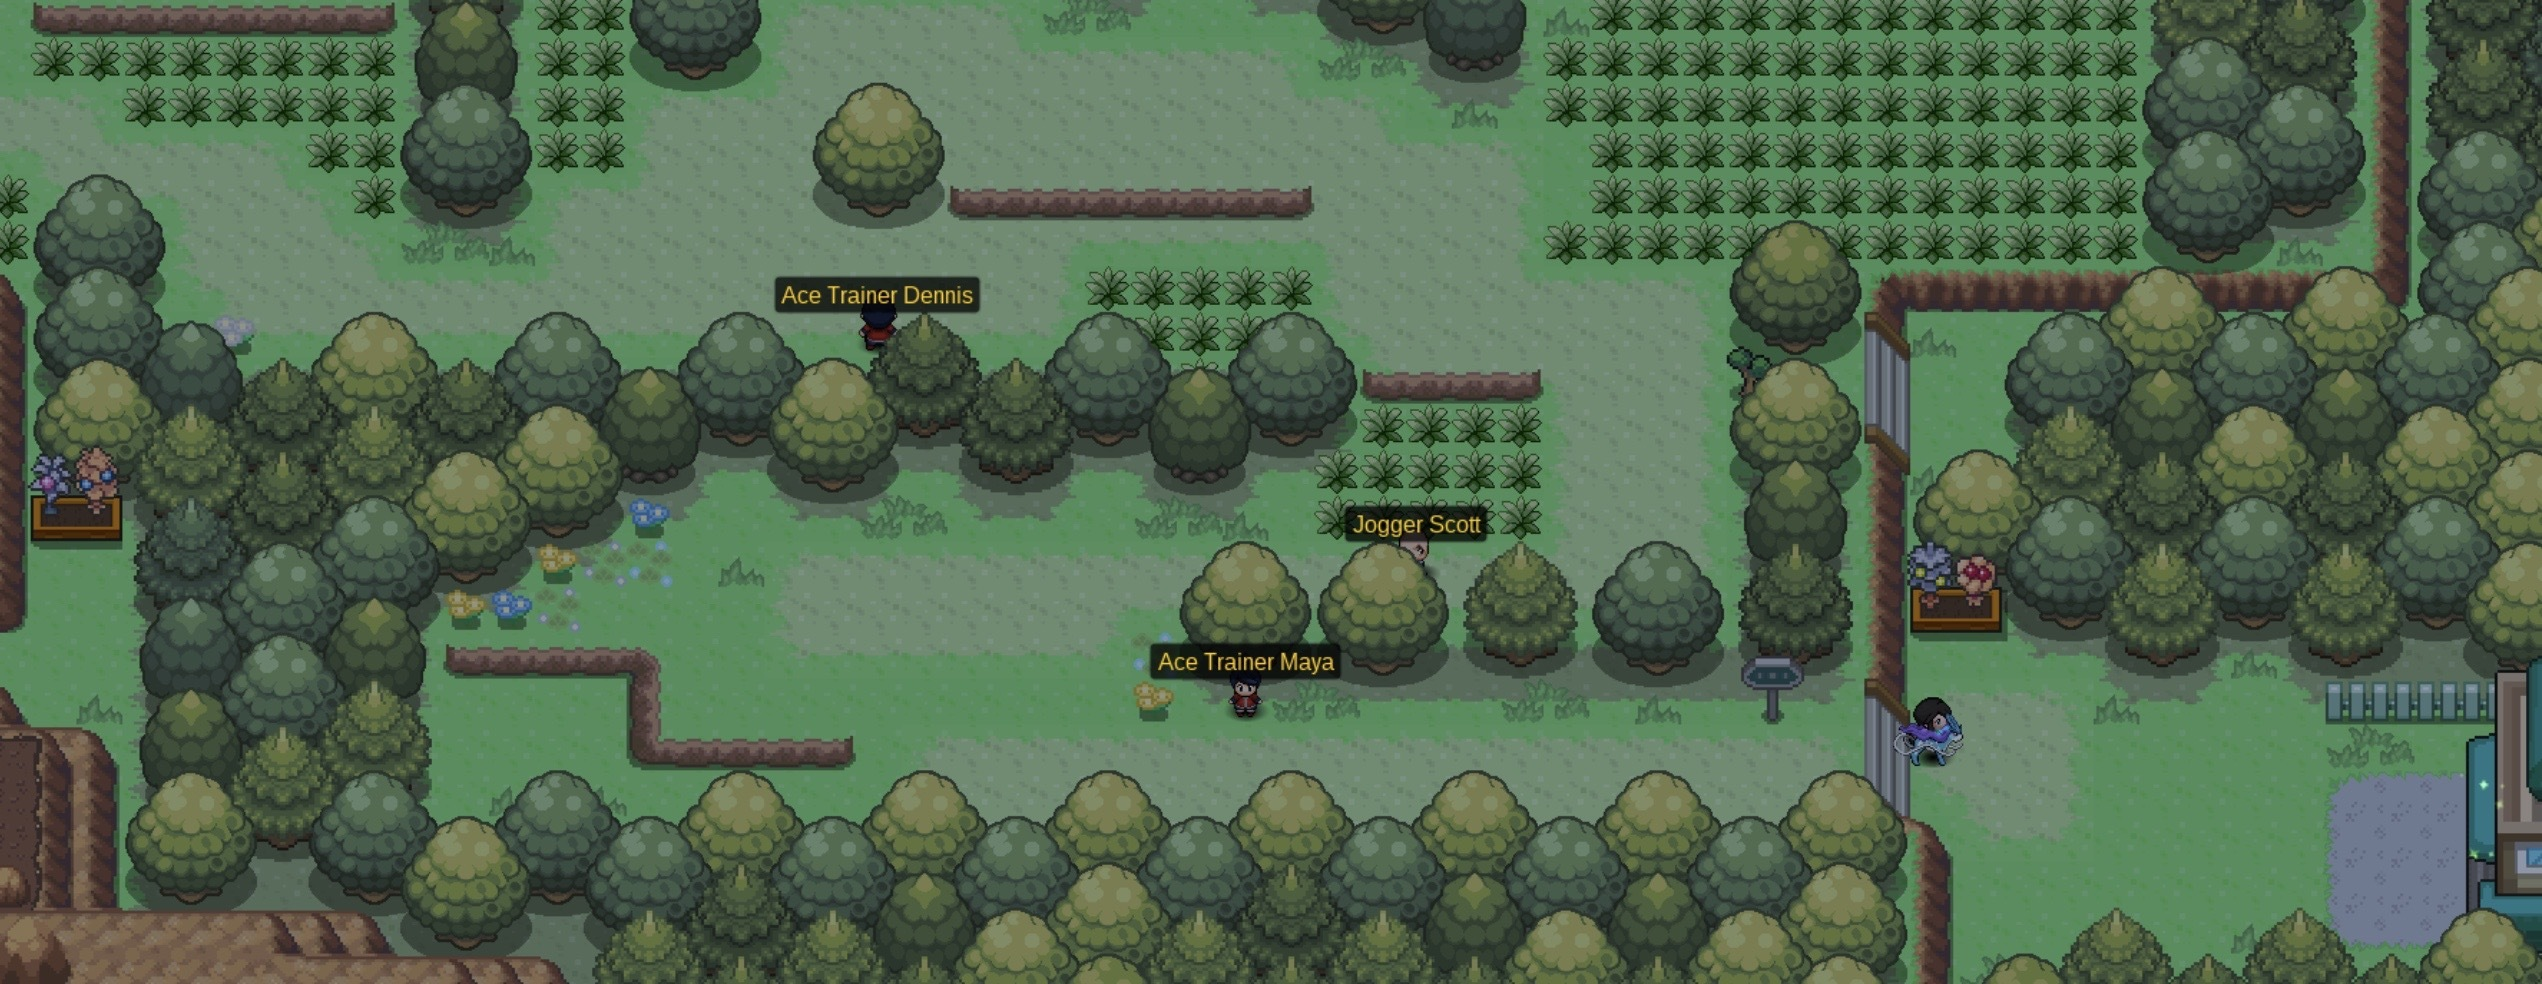
\includegraphics[width=\textwidth]{walkthrough/Sinnoh/Route_215}

\input{routes/Sinnoh/Route_215/Wild_Pokémon_(Land)}
\begin{longtable}{|| l l l l ||}%
\hline%
&Rare Candy&1&Not respawnable\\%
\hline%
&Revive&1&Not respawnable\\%
\hline%
&Full Heal&1&Not respawnable\\%
\hline%
&Pecha Berry&1{-}3&3 days\\%
\hline%
&Oran Berry&1{-}3&3 days\\%
\hline%
&Sitrus Berry&1{-}3&3 days\\%
\hline%
&Leppa Berry&1{-}3&3 days\\%
\hline%
\endhead%
\hline%
\caption{Items in Route 215}%
\label{tab:Route215Items}%
\end{longtable}

\subsubsection{Veilstone City}\label{subsubsec:veilstone-city}
Finally we are in the city.

Go to the gym and talk with dawn and then enter the gym.
In this gym we need to get two scrolls to be able to battle with the Leader.
Its always random so you need to battle with all trainers.
And be ready to battle with the leader.

\subsubsection{Veilstone City Gym}\label{subsubsec:veilstone-city-gym}
Maylene uses Fighting-type Pokemon.
Beat her and get the Cobble Badge.

\subsubsection{Dawn and After}\label{subsubsec:dawn-and-after}
Beat the gym and then you will find Dawn in the door.
She wil tell us that some grunts of the team galactic stole her pokedex and we need to help her.
Go to the north of the city and you will find Dawn with some Galactic Grunts.
Help her and be ready to battle.
After the battle, Talk with Dawn again and she will tell us to go to Pastoria City.

\subsection{Path to Pastoria City}\label{subsec:path-to-pastoria-city}

\subsubsection{Route 214}\label{subsubsec:route_214}

To go to Pastoria City you need to go to Route 214 in the south and follow all the routes.

\input{routes/Sinnoh/Route_214/Wild_Pokémon_(Land)}
\input{routes/Sinnoh/Route_214/Wild_Pokémon_(Water)}
\begin{longtable}{|| l l l l ||}%
\hline%
&Razor Fang&x 1&Not respawnable\\%
\multicolumn{4}{||m{\textwidth}||}{On the southmost tall grass maze in the west path.}%
\hline%
&Max Potion&x 1&Not respawnable\\%
\multicolumn{4}{||m{\textwidth}||}{Past the lake in the north-east corner. Requires Surf.}%
\hline%
&Sitrus Berry&x 1{-}2&3 days\\%
\multicolumn{4}{||m{\textwidth}||}{Berry Trees in the north-east of the route. There are two of them.}%
\hline%
&Cheri Berry&x 1{-}3&3 days\\%
\multicolumn{4}{||m{\textwidth}||}{Berry Tree in the north-east of the route.}%
\hline%
&Rawst Berry&x 1{-}2&3 days\\%
\multicolumn{4}{||m{\textwidth}||}{Berry Tree in the north-east of the route.}%
\hline%
\endhead%
\hline%
\caption{Items in Route 214}%
\label{tab:Route214Items}%
\end{longtable}

\subsubsection{Route 213}\label{subsubsec:route_213}

\paragraph{Valor Lakefront} For now the Lake itself is blocked from access, so
we are quickly passing through the Lakefront as we continue through Route 213.

\input{routes/Sinnoh/Route_213/Wild_Pokémon_(Land)}
\input{routes/Sinnoh/Route_213/Wild_Pokémon_(Water)}
\begin{longtable}{|| l l l l ||}%
\hline%
&Water Stone&x 1&Not respawnable\\%
\multicolumn{4}{||m{\textwidth}||}{On a mini-island in the far east, at the end of the southmost path. Requires Surf.}%
\hline%
&TM55 — Roar&x 1&Not respawnable\\%
\multicolumn{4}{||m{\textwidth}||}{On top of the hill in the middle of the route. Requires Rock Climb.}%
\hline%
&PP Up&x 1&Not respawnable\\%
\multicolumn{4}{||m{\textwidth}||}{Hidden item. On the closest palm tree north of Dr. Footstep’s House on the beach.}%
\hline%
&Big Pearl&x 1&Not respawnable\\%
\multicolumn{4}{||m{\textwidth}||}{Hidden item. On the south-eastmost small rock on the island in the south-east corner of the route. Requires Surf.}%
\hline%
&Pecha Berry&x 1{-}3&3 days\\%
\multicolumn{4}{||m{\textwidth}||}{Berry Tree next to the Pastoria City entrance.}%
\hline%
&Cheri Berry&x 1{-}3&3 days\\%
\multicolumn{4}{||m{\textwidth}||}{Berry Tree next to the Pastoria City entrance.}%
\hline%
&Leppa Berry&x 1{-}2&3 days\\%
\multicolumn{4}{||m{\textwidth}||}{Berry Tree next to the Pastoria City entrance.}%
\hline%
&Sitrus Berry&x 1{-}2&3 days\\%
\multicolumn{4}{||m{\textwidth}||}{Berry Tree next to the Pastoria City entrance.}%
\hline%
\endhead%
\hline%
\caption{Items in Route 213}%
\label{tab:Route213Items}%
\end{longtable}

\subsection{Pastoria Gym}\label{subsec:pastoria-gym}

\subsubsection{Pastoria City}\label{subsubsec:pastoria-city}
Go to the gym and get ready to battle with trainers and the leader.

\paragraph{Notables}\label{par:notables-pastoria-city}

\begin{itemize}
    \item TM Tutor - Hone Claws \emph{(Requires Surf)}
\end{itemize}

\subsubsection{Pastoria City Gym}\label{subsubsec:pastoria-city-gym}
Wake uses Water-type Pokemon.
Beat him and you will get the Fen Badge and now you can use Surf.

\subsection{Path to Celestic Town}\label{subsec:path-to-celestic-town}

\subsubsection{Cynthia and Cyrus}\label{subsubsec:cynthia-and-cyrus}
After you beat the gym, Go to the north of Pastoria City
and you will find a Galatic Grunt there you need to follow him though routes 213
and Valor Lakefront you need to beat him.
Now go up and talk with Cynthia, She will ask us to give the medicine to the
Psyducks in Route 210 and Give Old Charm to her Grandma in Celestic Town.

\input{routes/Sinnoh/Valor_Lakefront/Wild_Pokémon_(Land)}`
\begin{longtable}{|| l l l l ||}%
\hline%
&Sun Stone&x 1&Not respawnable\\%
\multicolumn{4}{||m{\textwidth}||}{In the south-east corner of the area. Requires to use Rock Climb on the east side of Route 213.}%
\hline%
&TM42 — Dream Eater&x 1&Not respawnable\\%
\multicolumn{4}{||m{\textwidth}||}{At the end of the western path, which must be entered from Route 213. Requires Rock Climb.}%
\hline%
\endhead%
\hline%
\caption{Items in Valor Lakefront}%
\label{tab:ValorLakefrontItems}%
\end{longtable}

\subsubsection{Route 212 South}\label{subsubsec:route-212-(south)}
We need to head to Route 210, so we might as well explore Route 212 on the way.
This area has plenty of trainers to work on.

\input{routes/Sinnoh/Route_212_South/Wild_Pokémon_(Land)}
\input{routes/Sinnoh/Route_212_South/Wild_Pokémon_(Water)}
\begin{longtable}{|| l l l l ||}%
\hline%
&Stardust&x 1&7 days\\%
\multicolumn{4}{||m{\textwidth}||}{In the south-east corner of the swamp part, south of Ranger Taylor.}%
\hline%
&Dawn Stone&x 1&Not respawnable\\%
\multicolumn{4}{||m{\textwidth}||}{At the end of the path north of Pastoria City’s entrance.}%
\hline%
\endhead%
\hline%
\caption{Items in Route 212 South}%
\label{tab:Route212SouthItems}%
\end{longtable}

\subsubsection{Route 212 North}\label{subsubsec:route-212-north}
Plenty of trainers to level up on.
This area also contains the Pokemon Mansion.

\paragraph{Pokemon Mansion}
- Celeste will give you 5 Ultra Balls if you beat her.
- There is a Big Nugget in one of the rooms.
- There is a Rich Kid who will give you a Rare Candy for beating him.
- There are 3 Super Potions on the right side.

\input{routes/Sinnoh/Route_212_North/Wild_Pokémon_(Land)}
\input{routes/Sinnoh/Route_212_North/Wild_Pokémon_(Water)}
\begin{longtable}{|| l l l l ||}%
\hline%
&TM61 — Sunny Day&x 1&Not respawnable\\%
\multicolumn{4}{||m{\textwidth}||}{Beyond a ledge in the middle west of the route. Requires either Surf or Cut.}%
\hline%
&Hyper Potion&x 3&Not respawnable\\%
\multicolumn{4}{||m{\textwidth}||}{Hidden item. On one of the plants slightly south-west from the Pokemon Mansion’s entrance door.}%
\hline%
&Pecha Berry&x 1{-}3&3 days\\%
\multicolumn{4}{||m{\textwidth}||}{Berry Tree west of the entrance to the Pokemon Mansion front yard.}%
\hline%
&Oran Berry&x 1{-}3&3 days\\%
\multicolumn{4}{||m{\textwidth}||}{Berry Tree west of the entrance to the Pokemon Mansion front yard.}%
\hline%
&Hondew Berry&x 3{-}9&4 days\\%
\multicolumn{4}{||m{\textwidth}||}{Berry Tree in the south-west corner. Requires Surf.}%
\hline%
&Qualot Berry&x 3{-}9&4 days\\%
\multicolumn{4}{||m{\textwidth}||}{Berry Tree in the south-west corner. Requires Surf.}%
\hline%
\endhead%
\hline%
\caption{Items in Route 212 North}%
\label{tab:Route212NorthItems}%
\end{longtable}

\subsubsection{Route 210 (North)}\label{subsubsec:route-210-(north)}
Give the medicine to the Psyducks to access Route 210 North.

\subsubsection{Celestic Town}\label{subsubsec:celestic-town}
In celestic Town we need to beat the Galatic Grunt blocking the cave.
After beating the Grunt, Cynthia's Grandma will appear behind you
and you need to give her the old charm.
Now enter in the cave and talk with this fossil, Cyrus will appear and be ready to the battle.

\paragraph{Notables}\label{par:notables-celestic}

\begin{itemize}
    \item Move Tutor: Magic Room
    \item Move Tutor: Trick Room
    \item Move Tutor: Magic Coat
    \item Item Maniac
\end{itemize}

\subsubsection{Route 211 (East)}\label{subsubsec:route_211_(east)}
Before we head back to Hearthome City let's clear out some random trainers to
the west of Celestic Town.

% \input{routes/Sinnoh/Route_211/Wild_Pokémon_(Diggable_Patches)}
\begin{longtable}{|| l l l l ||}%
\hline%
&TM62 — Taunt&x 1&Not respawnable\\%
\multicolumn{4}{||m{\textwidth}||}{Below the southmost bridge in the west part. Requires Rock Smash.}%
\hline%
&Ultra Ball&x 1&Not respawnable\\%
\multicolumn{4}{||m{\textwidth}||}{Hidden item. On the tree in the north-west corner of the west side of the route.}%
\hline%
&TM29 — Psychic&x 1&Not respawnable\\%
\multicolumn{4}{||m{\textwidth}||}{In the middle of the grass south of the east part.}%
\hline%
&Carbos&x 1&Not respawnable\\%
\multicolumn{4}{||m{\textwidth}||}{In the north-west corner of the east part. Requires Rock Smash.}%
\hline%
&Ultra Ball&x 1&Not respawnable\\%
\multicolumn{4}{||m{\textwidth}||}{Hidden item. On the tree in the north-west corner of the west side of the route.}%
\hline%
&Leppa Berry&x 1{-}2&3 days\\%
\multicolumn{4}{||m{\textwidth}||}{Berry Trees next to the Celestic Town entrance. There are 3 of them.}%
\hline%
\endhead%
\hline%
\caption{Items in Route 211}%
\label{tab:Route211Items}%
\end{longtable}

\subsubsection{Mt. Coronet (Center)}\label{subsubsec:mt.-coronet-(center)}
Then enter Mt. Coronet (Center).
Just a couple of Trainers here we can fight.
Otherwise we are blocked by the Onix and Steelix.

\input{routes/Sinnoh/Mt._Coronet_North/Wild_Pokémon_(Mt._Coronet_Center)}


\subsection{Back to Hearthome City}\label{subsec:back-to-hearthome-city}

\subsubsection{Route 209}
From Celestic Town head east to Route 210 and then South through
Solaceon Town to Route 209.

\subsubsection{Route 212}
Continue west to Hearthome City and then head south to Route 212
In Route 212 North, southwest of Pokemon mansion, surf west on the pond and
you can collect some Berries: Qualot and Hondew.
Continue South to Pastoria City.

\subsubsection{Pastoria City}
You can now use Surf to reach the TM Tutor for Hone Claws.
Use Surf near the guy who stands at the middle of the city.
Surf east and stop surfing between two trees.
Head inside and you can find the item Mystic Water,
which boosts the power of the Water-type moves of a Pokémon that holds it.

\subsubsection{Route 213}
Head east out of Pastoria City
Surf southeast from Fisherman Kenneth (the fisherman that fought you).
Head into the sea between two rocks.
There are a few Trainers for you to fight and some items for you to collect in that area.
- Big Pearl in bottom-right rock near Sailor Paul.
- Water Stone on a sandbar.

\subsubsection{Route 214}
Keep going North through Valor Lakefront to Route 214.
In the northern area there is a small pond you can surf across to reach
a Max Potion.

\subsubsection{Mt. Coronet (South)}
Head to the south.
Go up the stairs that leads to another pond.
Surf east, and you can get the Dawn Stone.
Upstairs you can find Rock Slide.
There is a Galactic Grunt protecting a passage way but you cannot access yet.

\begin{longtable}{|| l l l l ||}%
\hline%
&Dusk Stone&x 1&Not respawnable\\%
\multicolumn{4}{||m{\textwidth}||}{In the south-east corner of Mt. Coronet South. Requires Surf.}%
\hline%
&TM48 — Rock Slide&x 1&Not respawnable\\%
\multicolumn{4}{||m{\textwidth}||}{In the south-west corner of Mt. Coronet 2F.}%
\hline%
&Escape Rope&x 1&Not respawnable\\%
\multicolumn{4}{||m{\textwidth}||}{Near the north-west corner of Mt. Coronet 2F, next to the Rock Smash rocks.}%
\hline%
&Hyper Potion&x 2&Not respawnable\\%
\multicolumn{4}{||m{\textwidth}||}{In the north-east corner of the main part of Mt. Coronet 2F.}%
\hline%
&Star Piece&x 1&Not respawnable\\%
\multicolumn{4}{||m{\textwidth}||}{In the east-most room of Mt. Coronet 2F, accessible from the eastmost ladder of 3F.}%
\hline%
&Revive&x 1&Not respawnable\\%
\multicolumn{4}{||m{\textwidth}||}{Hidden item. On the rock adjacent to the stairs in Mt. Coronet 3F.}%
\hline%
\endhead%
\hline%
\caption{Items in Mt. Coronet South}%
\label{tab:Mt.CoronetSouthItems}%
\end{longtable}

\subsubsection{Route 206}
The area under the biking road is now accessible via Surf.
There are a number of trainers to defeat here.
There is a Rare Candy to be obtained in the top left.

\input{routes/Sinnoh/Route_206/Wild_Pokémon_(Land)}
\begin{longtable}{|| l l l l ||}%
\hline%
&Rare Candy&1&7 days\\%
\hline%
&Leftovers&1&Not respawnable\\%
\hline%
&Burn Heal&1&Not respawnable\\%
\hline%
\endhead%
\hline%
\caption{Items in Route 206}%
\label{tab:Route206Items}%
\end{longtable}

\subsubsection{Wayward Cave}

Wayward Cave has the main visible entrance, and another secret entrance under
the bridge.
The secret entrance leads to TM Tutor Tri Attack.

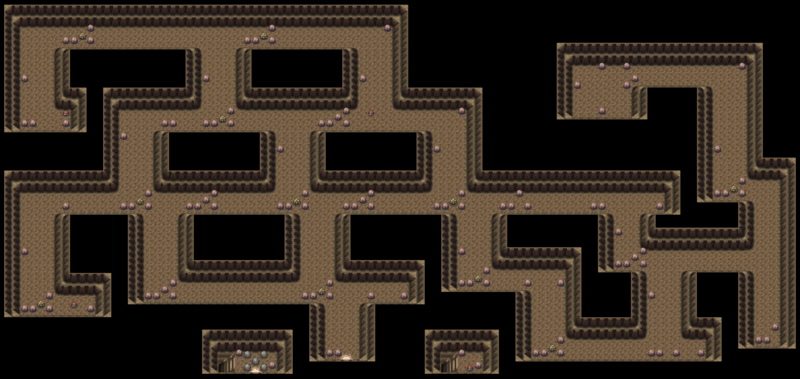
\includegraphics[width=\textwidth]{walkthrough/Sinnoh/wayward-cave}

\input{routes/Sinnoh/Wayward_Cave/Wild_Pokémon_(Wayward_Cave)}

\subsubsection{Hearthome City Gym}\label{subsubsec:hearthome-city-gym}
The Gym in Hearthome City is next to where you battled with Barry next to Route 209.
Once in Hearthome City go to the gym and be ready to battle.
This gym is a bit hard without Flash but you can catch a Roselia in Route 212
and it can learn Flash.
I made this tutorial to this gym maze.

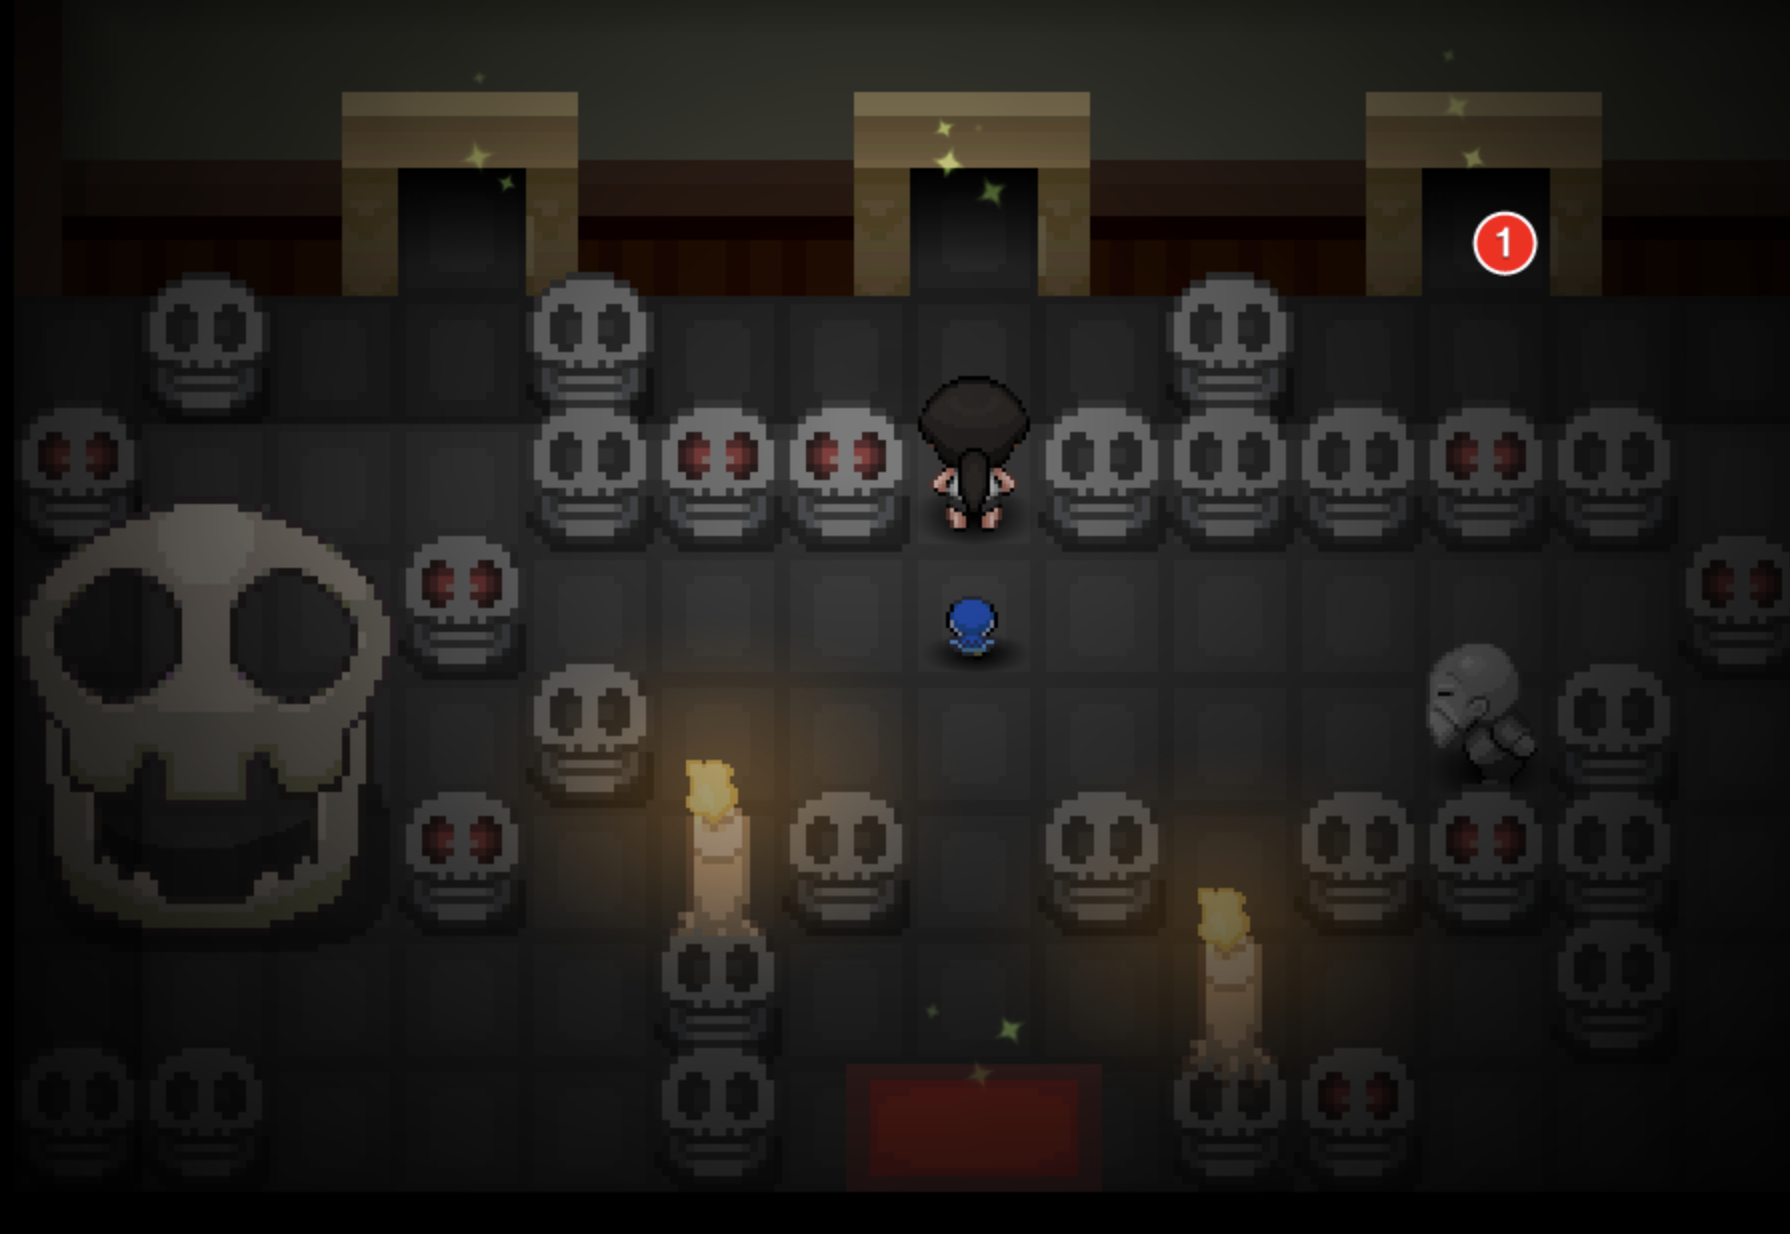
\includegraphics[width=\textwidth]{walkthrough/Sinnoh/hearthome_gym_1}
And the next part:

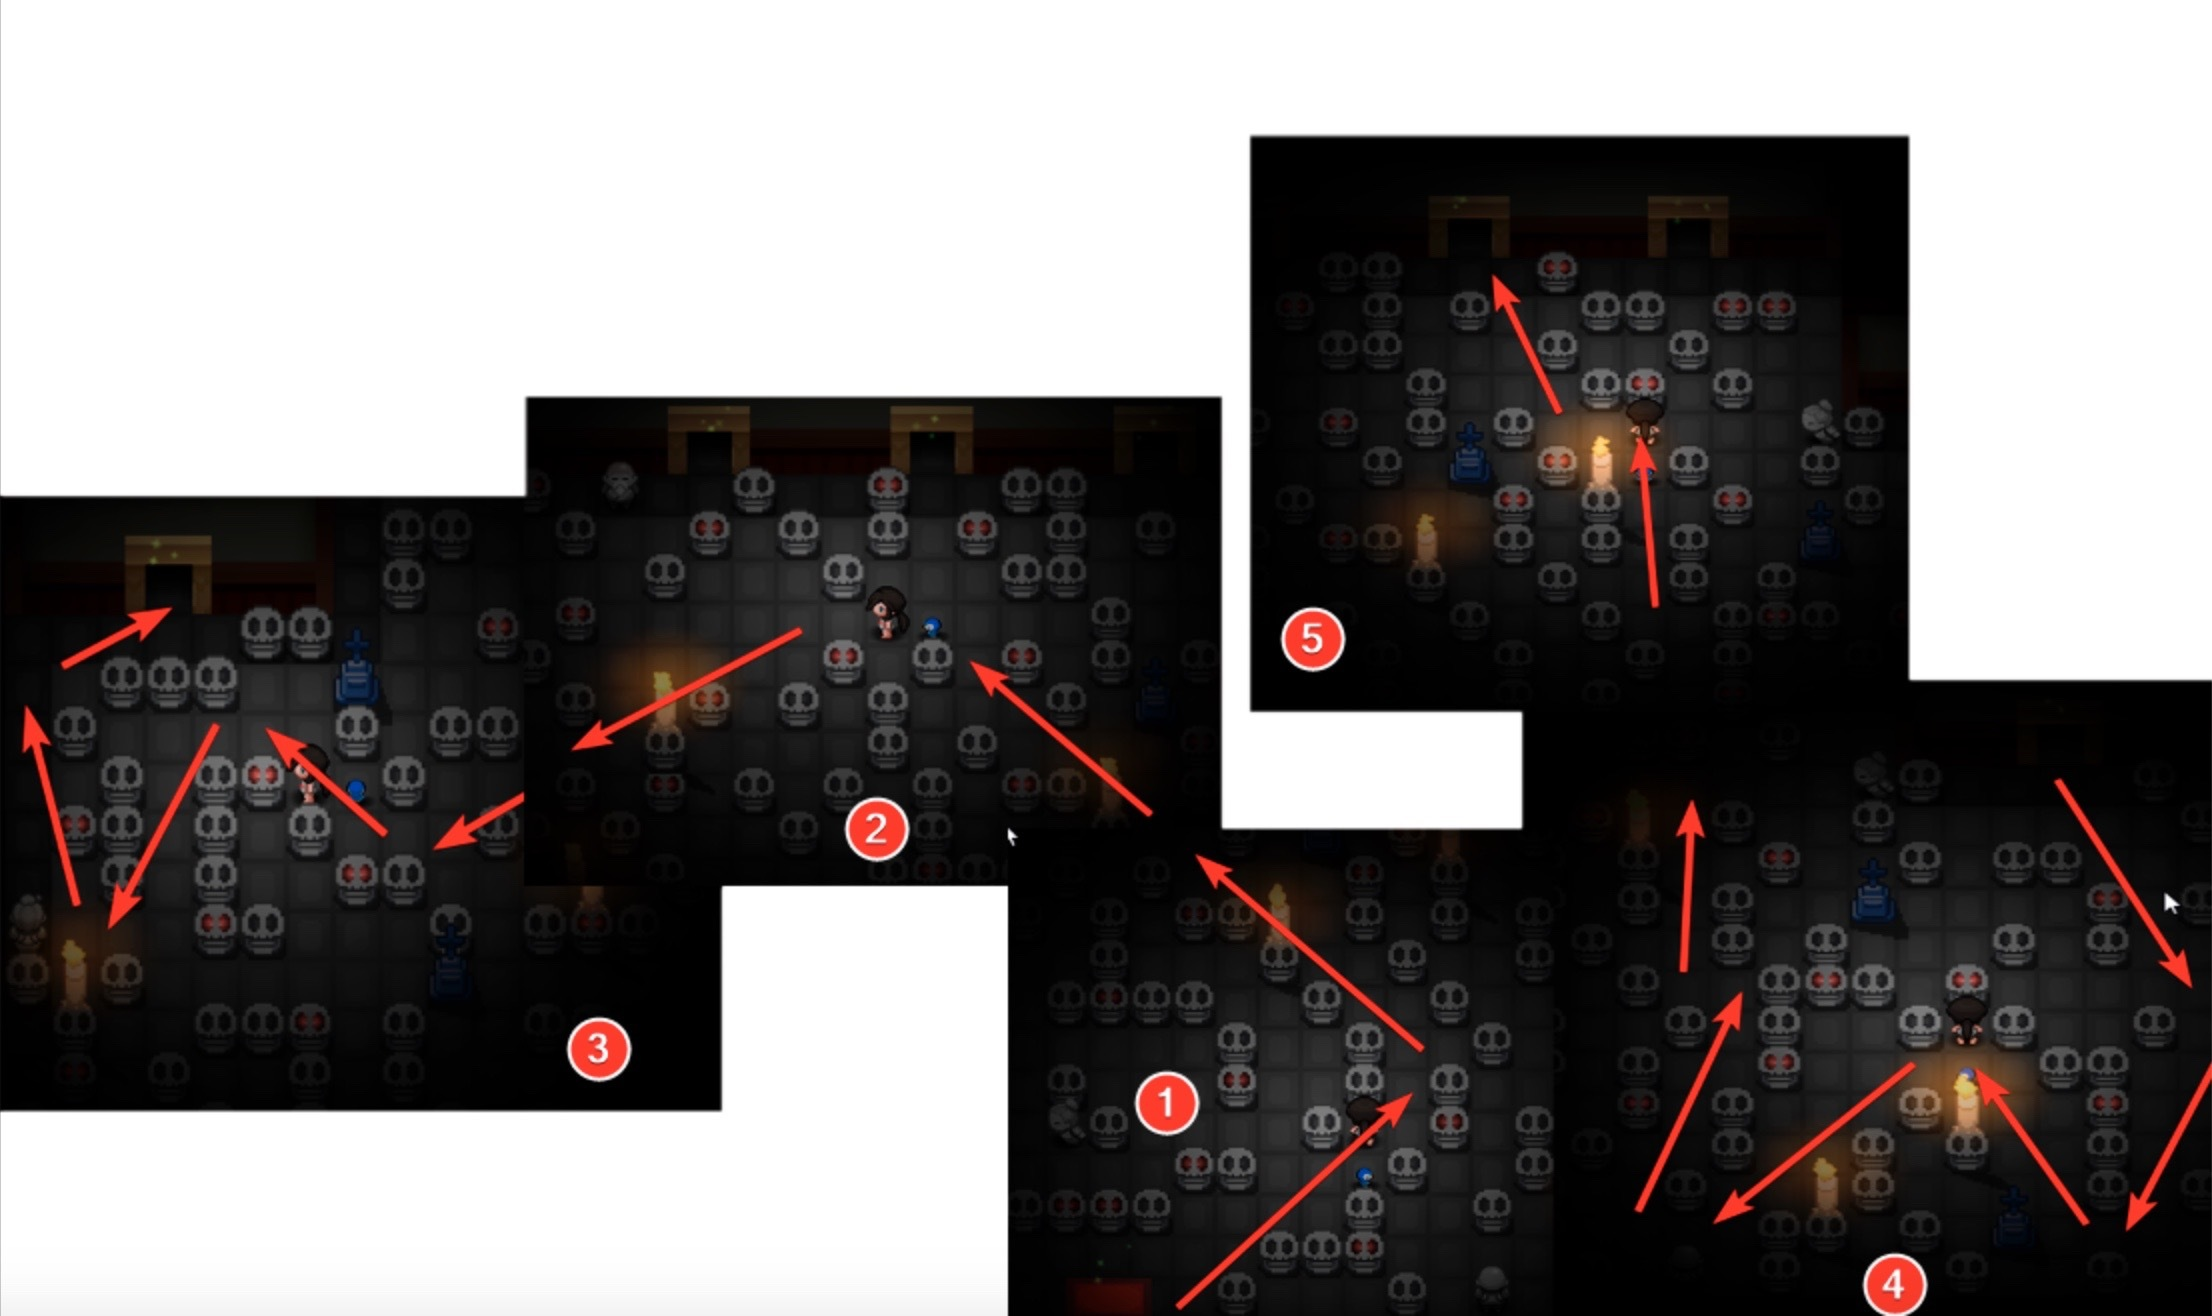
\includegraphics[width=\textwidth]{walkthrough/Sinnoh/hearthome_gym_2}
Fantina uses Ghost-type Pokemon.
Beat her and you will get the Relic Badge.
She will tell us to visit the Library in Canalave City.

\subsection{Fuego Ironworks}\label{subsec:fuego-ironworks}
Go to Route 205.
Remember the house south of Eterna Forest,
which you can take a rest and heal your Pokémon?
Head south from there and go down the stairs.
Turn west when you can.
You will see a river.
Now that you can use Surf, you can get through this river.
Keep travelling north, and this river will bring you to Fuego Ironworks.
Travelling south brings you to Valley Windworks.
Go to the north of the river.
You will see a patch of grass.
Go through it, and you will see a factory.

here are many Trainers inside.
You will also see something familiar if you have played
Pokémon FireRed and LeafGreen.
Yes, these are the spinners again.
Step on it, and you will spin in circles and travel in the direction
that the arrow of the spinner points to.
For example, if you step on a spinner with an arrow on it that points to the left,
you will spin to the left and keep going until you hit something or another spinner.

There are a few Trainers for you to fight.
Fight them, collect the items and use the spinners to go around.
Eventually you will reach the boiler and Mr. Fuego.
He will give you a Fire Stone.
Afterwards, collect TM35 (Flamethrower), and leave Fuego Ironworks.

There is an one-way exit east of Fuego Ironworks, which leads you back to Route 205.
Jump down the two ledges, and you will find yourself near the entrance of
Eterna Forest and the healing house.

\input{routes/Sinnoh/Fuego_Ironworks/Wild_Pokémon_(Land)}
\input{routes/Sinnoh/Fuego_Ironworks/Wild_Pokémon_(Water)}
\input{routes/Sinnoh/Fuego_Ironworks/Wild_Pokémon_(Headbuttable_Trees)}
\begin{longtable}{|| l l l l ||}%
\hline%
&Burn Heal&1&Not respawnable\\%
\hline%
&Fire Stone&1&Not respawnable\\%
\hline%
&Rock Incense&1&Not respawnable\\%
\hline%
&Hyper Potion&2&Not respawnable\\%
\hline%
&TM85 — Flamethrower&1&Not respawnable\\%
\hline%
&Ultra Ball&1&Not respawnable\\%
\hline%
&Lum Berry&1{-}2&3 days\\%
\hline%
\endhead%
\hline%
\caption{Items in Fuego Ironworks}%
\label{tab:FuegoIronworksItems}%
\end{longtable}

\subsection{Canalave Gym}\label{subsec:canalave-gym}

\subsubsection{Back to Jubilife City}\label{subsubsec:back-to-jubilife-city}
Time to travel back to Jubilife City, by way of Route 208 to Route 218.

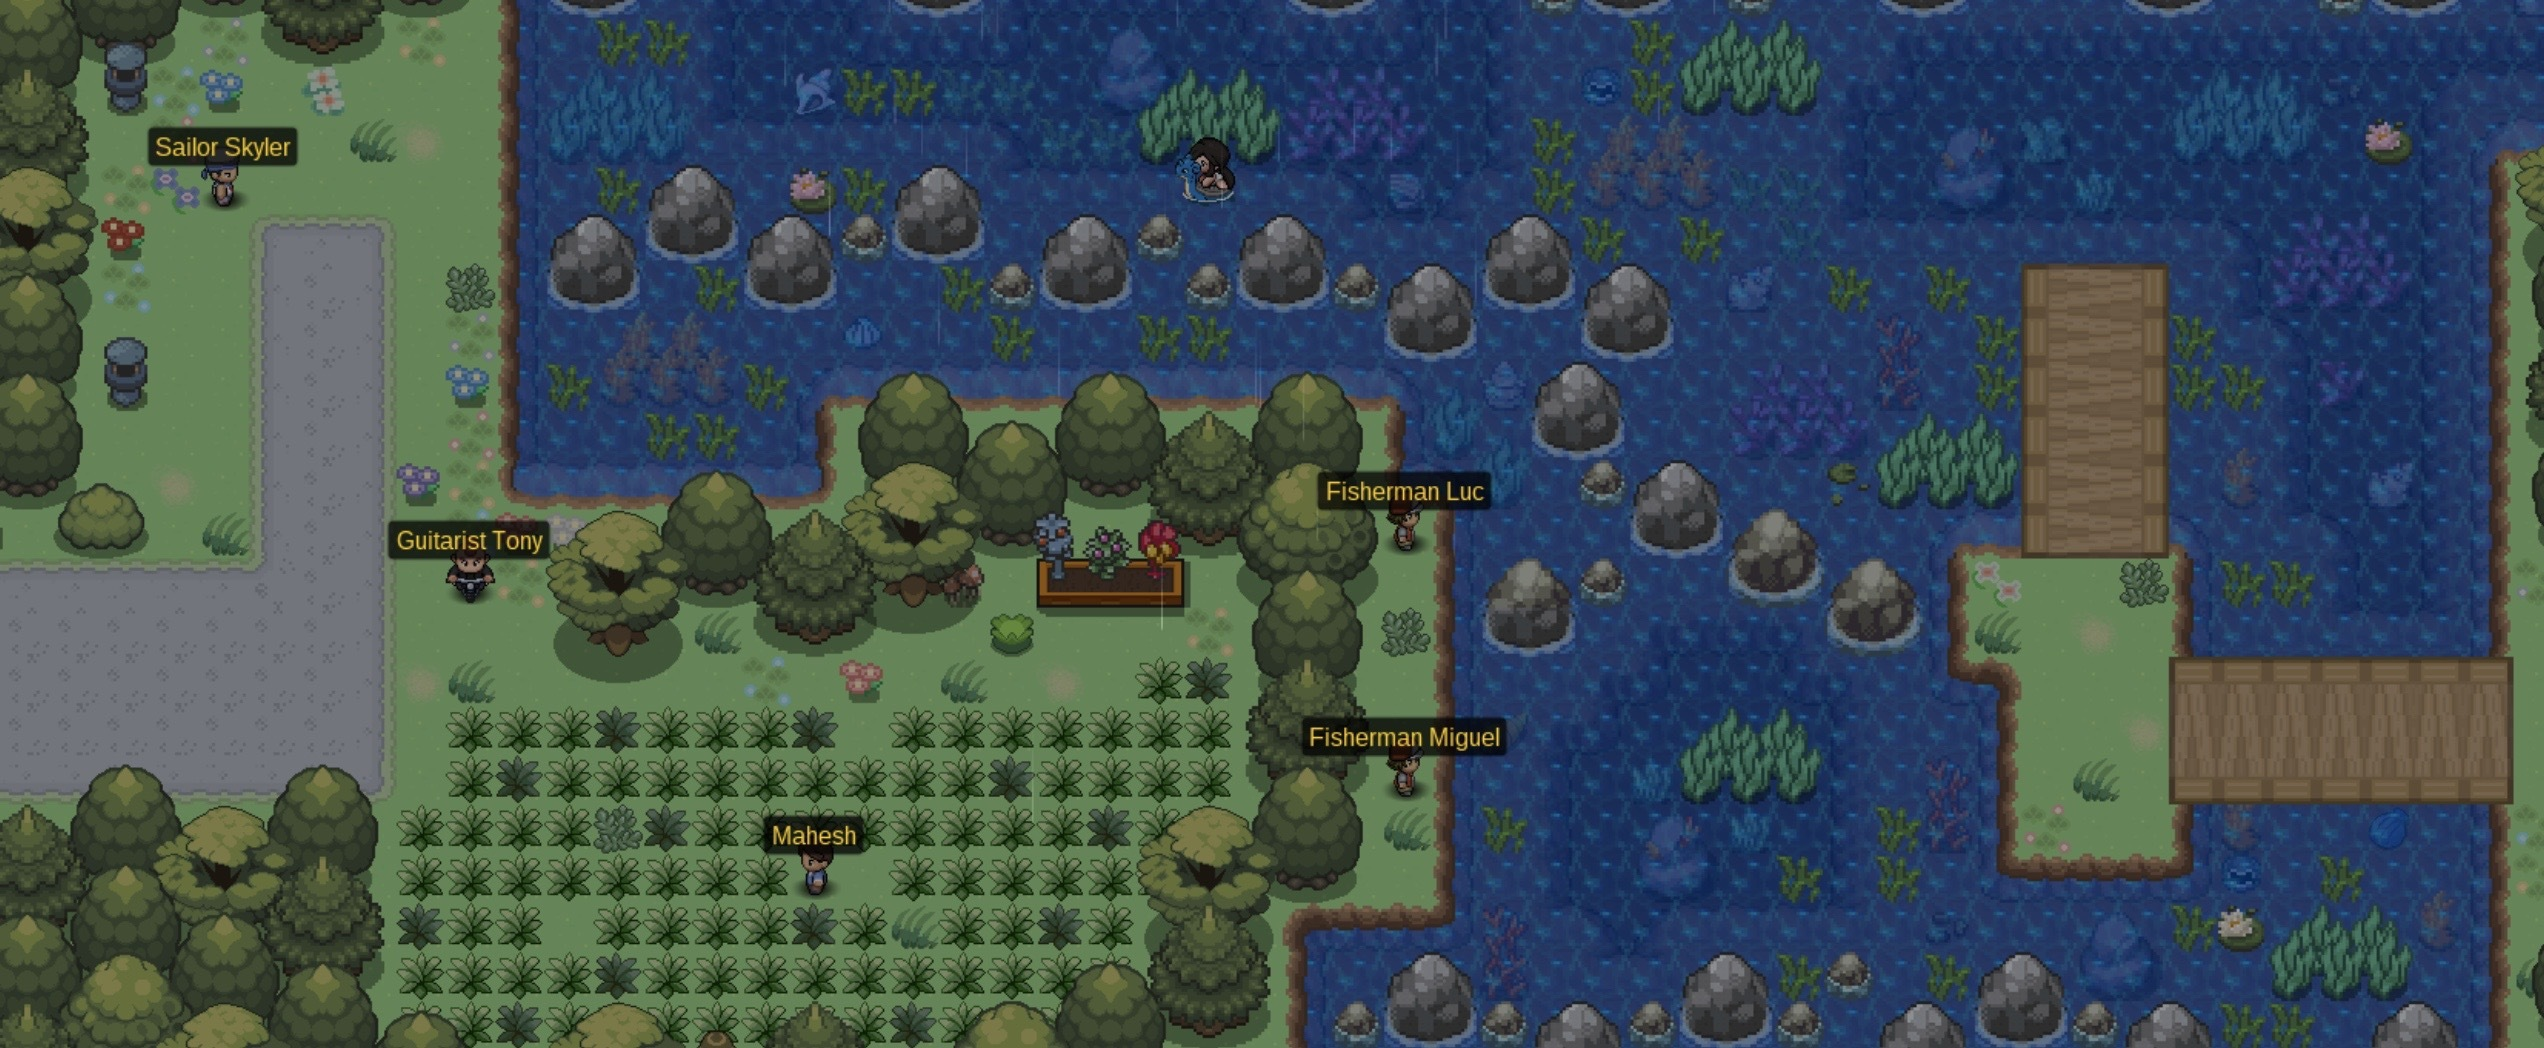
\includegraphics[width=\textwidth]{walkthrough/Sinnoh/Route_218}

\paragraph{Route 218}
Backtrack to Jubilife.
Go west to Route 218.
Surf to the top right to get a Rare Candy.
Then, head west.

\input{routes/Sinnoh/Route_218/Wild_Pokémon_(Water)}

\subsubsection{Canalave City}\label{subsubsec:canalave-city}
And finally we are in Canalave city.
Go to the gym and we are going to find barry blocking the way.
Talk with him and be ready to battle.
And now go to the gym.
This gym puzzle its easy so this time we dont need a tutorial.
Battle with trainers and beat the leader.
Byron uses Steel-type Pokemon.
Beat him and you will get the Mine badge.
He will tell us that we need to go to Snowpoint but first,
we are confronted by Barry again.

\subsubsection{Iron Island}\label{subsubsec:iron-island}
There is no PokeCenter on Iron Island so bring healing items or Escape Ropes to save time.

Iron Island is an island off the northwestern coast of Sinnoh.
It was once a prosperous ore mine, but was shut down after the ore reserves dried up.
Since then, it was kept open as a training area and habitat for wild Pokémon.

% \input{routes/Sinnoh/Iron_Island/Wild_Pokémon_(Iron_Island)}

\paragraph{1F}
Go down the right ladder first.

\input{routes/Sinnoh/Iron_Island/Wild_Pokémon_(Iron_Island_1F)}

\paragraph{B1F}
Go down the right ladder first.

\input{routes/Sinnoh/Iron_Island/Wild_Pokémon_(Iron_Island_B1F_L)}
\input{routes/Sinnoh/Iron_Island/Wild_Pokémon_(Iron_Island_B1F_R)}

\paragraph{B2F}
On the right side, it's just a bunch of trainers.
On the left side, you can navigate to the entrance to the Exit Room.

\input{routes/Sinnoh/Iron_Island/Wild_Pokémon_(Iron_Island_B2F_L)}
\input{routes/Sinnoh/Iron_Island/Wild_Pokémon_(Iron_Island_B2F_R)}

\paragraph{Exit Room}
You can get TM Smart Strike here.

\input{routes/Sinnoh/Iron_Island/Wild_Pokémon_(Iron_Island_Exit_Room)}

\subsubsection{Canalave Gym}

\subsection{Prof Rowan and Trio Lakes}\label{subsec:prof-rowan-and-trio-lakes}
Go to the library in Canalave City and go to the second floor.
There we are going to find Prof Rowan with Dawn and Barry,
we need to help him to protect the Guardians.

\subsubsection{Lake Valor}\label{subsubsec:lake-valor}
Now go back to Pastoria City and go to Valor Lakefront.
Get ready to battle with a lot of members of Team Galatic.
Go to the Cave and beat Saturn.

\input{routes/Sinnoh/Lake_Valor/Wild_Pokémon_(Land)}
\input{routes/Sinnoh/Lake_Valor/Wild_Pokémon_(Water)}
\input{routes/Sinnoh/Lake_Valor/Wild_Pokémon_(Headbuttable_Trees)}

\subsubsection{Lake Verity}\label{subsubsec:lake-verity}
After beating Saturn we need to go and help Prof Rowan and Dawn in Lake Verity, Go back to Route 201 and go to the left.
Battle with Mars and beat him

\subsubsection{Mt. Coronet North}\label{subsubsec:mt.-coronet-north}
And finally we need to help Barry in Lake Acuity.
To get there we must go back to Eterna City and to the right, into Mt. Coronet Center.
Go up, then into the basement, then further up into Mt. Coronet North.
Eventually you will find an exit to Route 216.

\input{routes/Sinnoh/Mt._Coronet_North/Wild_Pokémon_(Mt._Coronet_North)}
\begin{longtable}{|| l l l l ||}%
\hline%
&Super Repel&x 1&Not respawnable\\%
\multicolumn{4}{||m{\textwidth}||}{Slightly north of Route 211’s western exit in Mt. Coronet Center. Requires Rock Smash.}%
\hline%
&PP Up&x 1&Not respawnable\\%
\multicolumn{4}{||m{\textwidth}||}{In the middle of the lake in Mt. Coronet B1F. Requires Surf.}%
\hline%
&Max Potion&x 2&Not respawnable\\%
\multicolumn{4}{||m{\textwidth}||}{At the end of the narrow path in the north-east of Mt. Coronet B1F. Requires Rock Smash.}%
\hline%
&Ultra Ball&x 3&Not respawnable\\%
\multicolumn{4}{||m{\textwidth}||}{Hidden item. After going down the stairs between the two westmost Galactic Grunts, on the closest accessible rock to the water in B1F. Requires Rock Smash.}%
\hline%
&HP Up&x 1&Not respawnable\\%
\multicolumn{4}{||m{\textwidth}||}{Hidden item. On the south-eastmost rock in Mt. Coronet North.}%
\hline%
&Eviolite&x 1&Not respawnable\\%
\multicolumn{4}{||m{\textwidth}||}{Directly south from the north entrance in Mt. Coronet Tunnel, in an area enclosed by Rock Smash rocks.}%
\hline%
\endhead%
\hline%
\caption{Items in Mt. Coronet North}%
\label{tab:Mt.CoronetNorthItems}%
\end{longtable}

\subsubsection{Route 216}\label{subsubsec:route-2162}
Now we are in Route 216, nothing important in this route just a lot of trainers.

\input{routes/Sinnoh/Route_216/Wild_Pokémon_(Land)}
\begin{longtable}{|| l l l l ||}%
\hline%
&TM13 — Ice Beam&1&Not respawnable\\%
\hline%
&Ice Heal&1&Not respawnable\\%
\hline%
\endhead%
\hline%
\caption{Items in Route 216}%
\label{tab:Route216Items}%
\end{longtable}

\subsubsection{Route 217}\label{subsubsec:route-217}
Same as Route 216, In route 217 We are going to find a lot of trainers

\input{routes/Sinnoh/Route_217/Wild_Pokémon_(Land)}
\begin{longtable}{|| l l l l ||}%
\hline%
&Protein&2&Not respawnable\\%
\hline%
&TM57 — Hail&1&Not respawnable\\%
\hline%
&Revive&2&Not respawnable\\%
\hline%
&Max Potion&2&Not respawnable\\%
\hline%
&Ice Stone&1&Not respawnable\\%
\hline%
\endhead%
\hline%
\caption{Items in Route 217}%
\label{tab:Route217Items}%
\end{longtable}

\subsubsection{Acuity Lakefront}\label{subsubsec:acuity-lakefront}
But at the north we are going to find This Team Galactic blocking the way.
We need to get the Icicle Badge first.
Go to the right and We are in Snowpoint City.

\input{routes/Sinnoh/Acuity_Lakefront/Wild_Pokémon_(Land)}
\begin{longtable}{|| l l l l ||}%
\hline%
&Reaper Cloth&x 1&Not respawnable\\%
\multicolumn{4}{||m{\textwidth}||}{Behind the large tree slightly west of the Lake Acuity entrance.}%
\hline%
&Ultra Ball&x 5&Not respawnable\\%
\multicolumn{4}{||m{\textwidth}||}{Hidden item. At the very end of the westmost path.}%
\hline%
&Focus Sash&x 1&Not respawnable\\%
\multicolumn{4}{||m{\textwidth}||}{Hidden item. On the small rock between the two trees in the north-east wall of the route.}%
\hline%
\endhead%
\hline%
\caption{Items in Acuity Lakefront}%
\label{tab:AcuityLakefrontItems}%
\end{longtable}

\subsubsection{Snowpoint City}\label{subsubsec:snowpoint-city}

\subsubsection{Lake Acuity}\label{subsubsec:lake-acuity}
Go back to Acuity Lakefront and now Lake Acuity is accessible.
Talk with Barry, He will tell us that
he lost and we need to go to Team Galactic HQ in Veilstone City!

\subsection{Team Galactic Headquarters}\label{subsec:team-galactic-headquarters}
Go back to Veilstone City and Talk with the guy in front of the HQ,
Beat him and he will give us the password!
Now go to the left of the city and enter this warehouse!
Use the password and go downstairs.
Follow the way until this room and take the Teleport!

\includegraphics[width=\textwidth]{walkthrough/Sinnoh/galactic-1}

Now follow the way again until this bin, Search in the bin and you will
find a paper with the pasword to open the next doors!

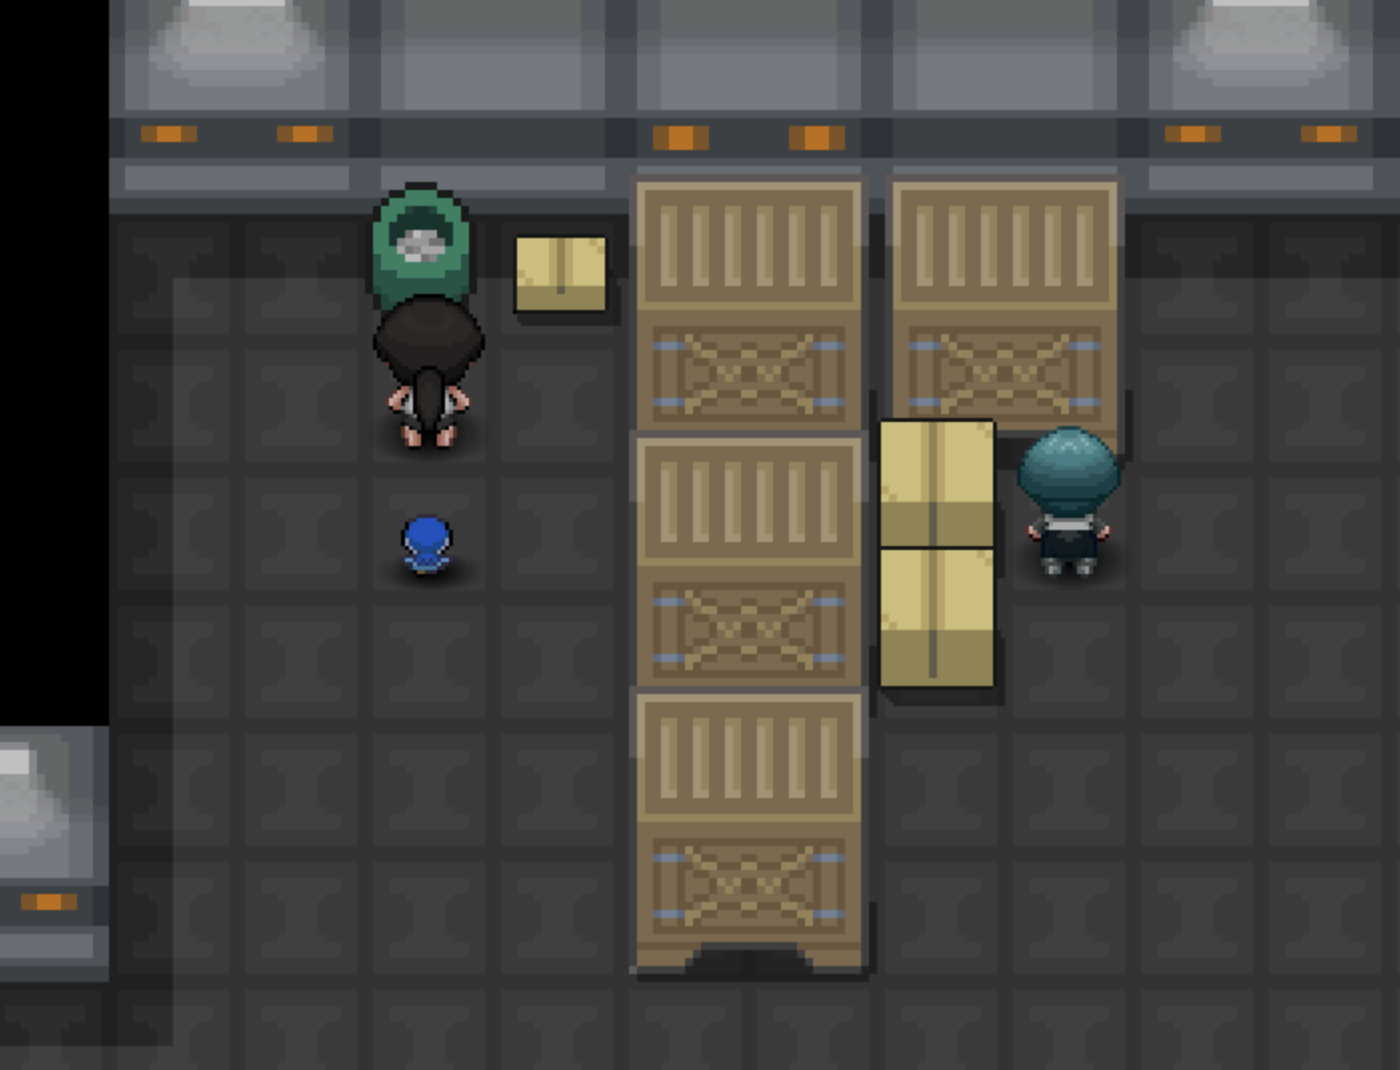
\includegraphics[width=\textwidth]{walkthrough/Sinnoh/galactic-2}

Now go back to the HQ and use the password to go up stairs!
Follow the way and use the teleporter in the room with a TV!

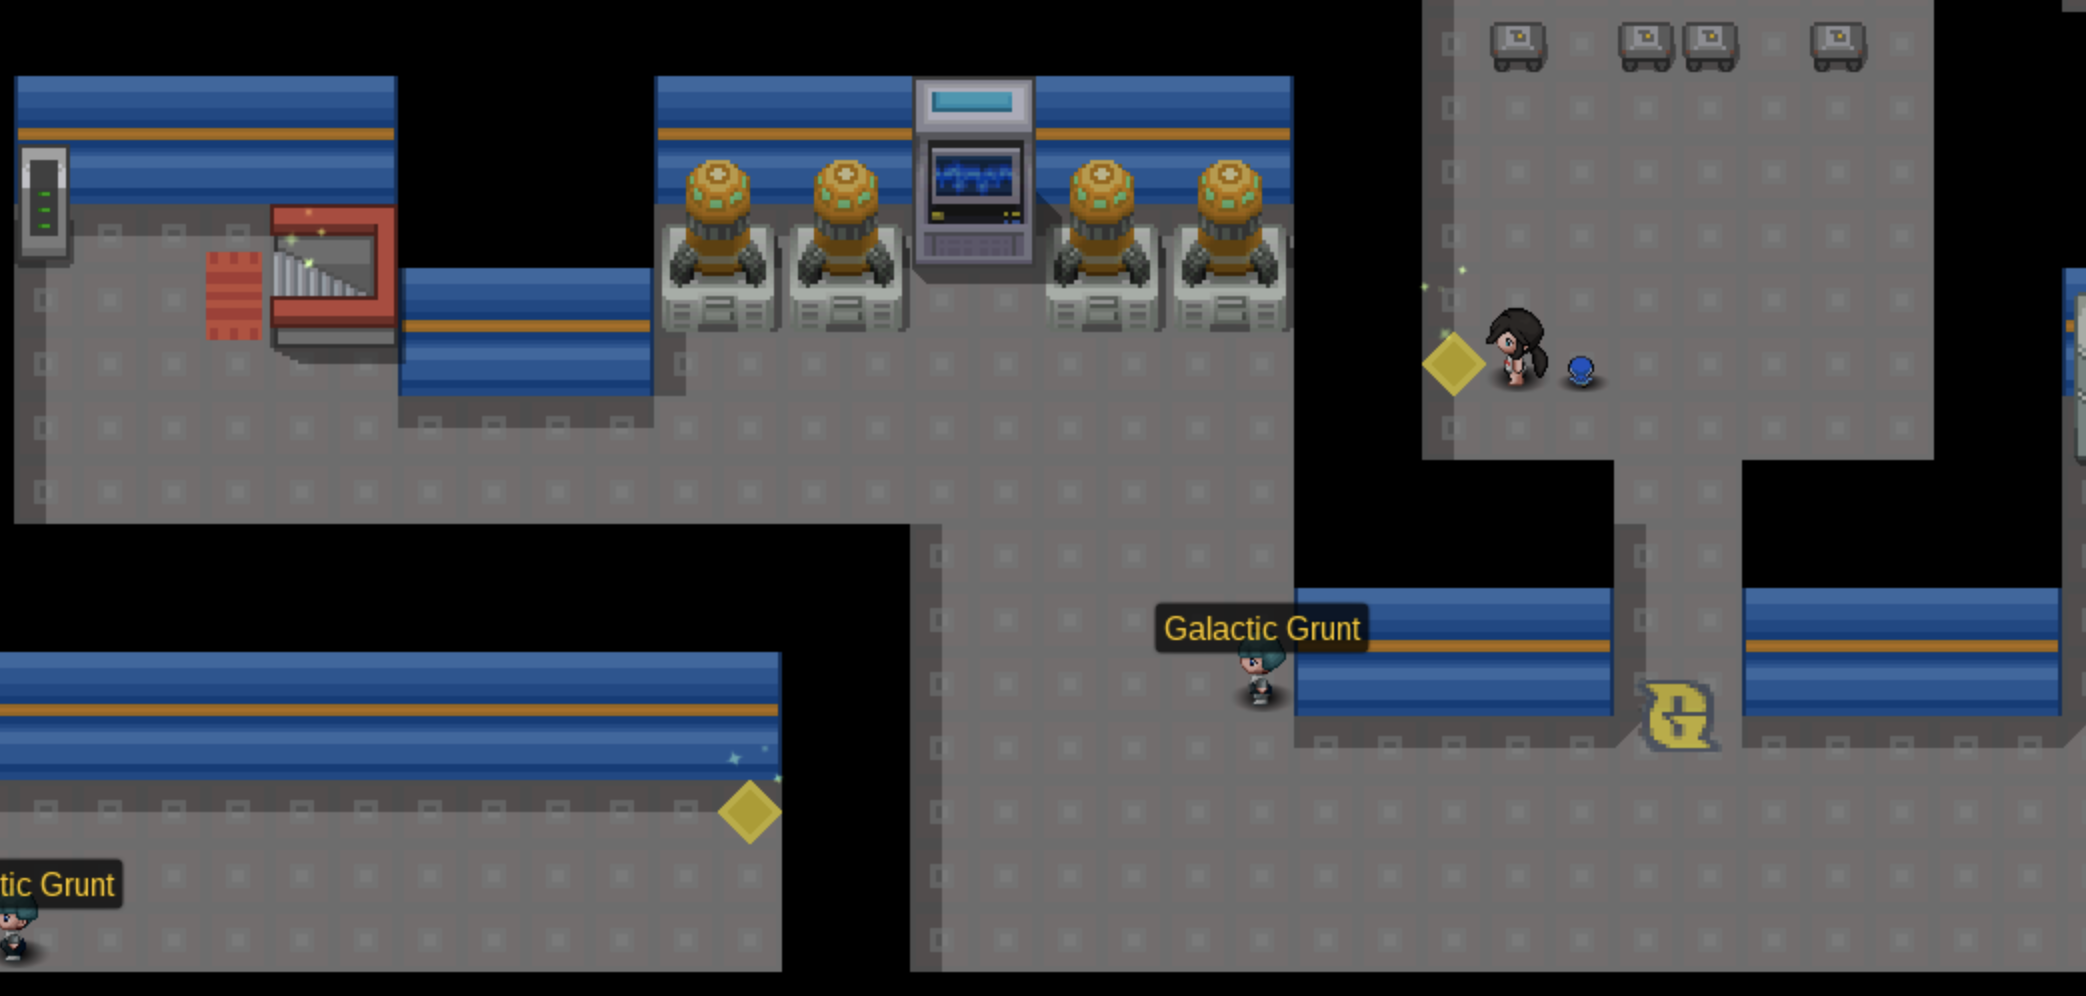
\includegraphics[width=\textwidth]{walkthrough/Sinnoh/galactic-3}

Now use the teleporter in the left!

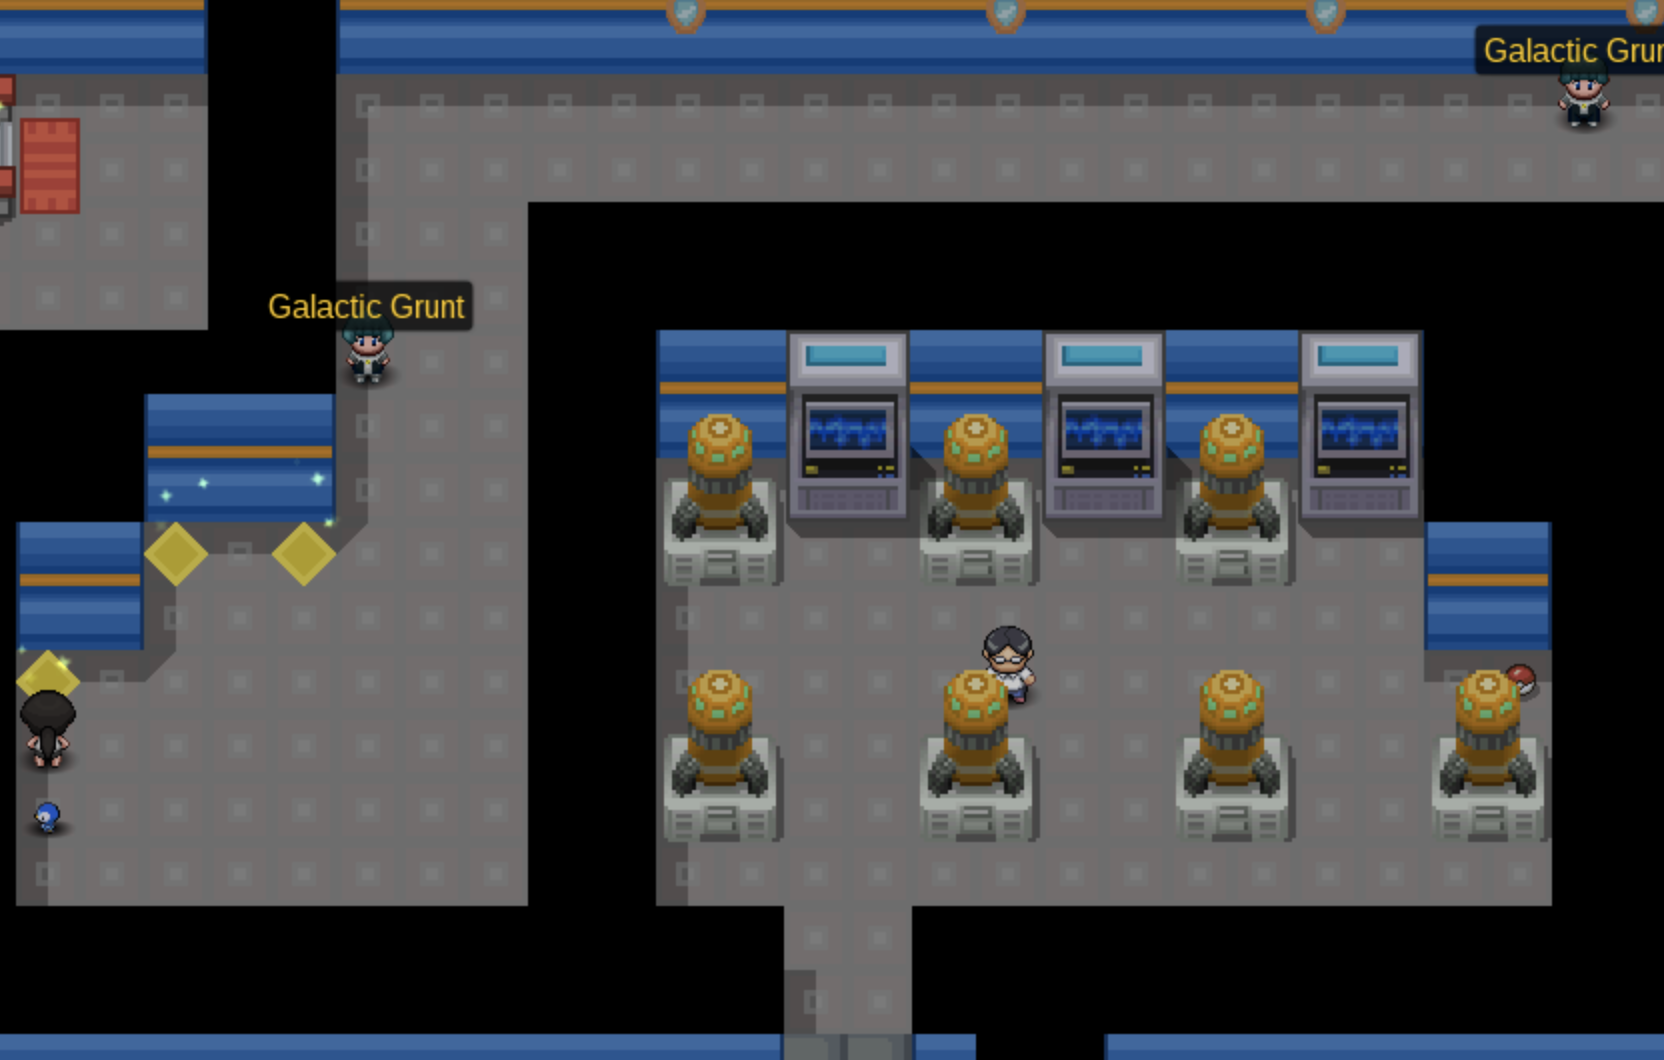
\includegraphics[width=\textwidth]{walkthrough/Sinnoh/galactic-4}

And finaly you will find Cyrus, Beat him!
After you beat him take the teleporter in the right!
And now be ready to battle with Saturn!
Beat him and now press the button in the machine!

\subsubsection{Mt. Coronet Summit}\label{subsubsec:back-to-mt.-coronet}
Now go back to Celestic Town and enter Mt. Coronet but this time go down!
Go to the top of the mountain and be ready for a lot of battles!
And finally we are in the top!, Talk with Cyrus and he will be
teleported to other dimension with Giratina!

\begin{longtable}{|| l l l l ||}%
\hline%
&Water Stone&x 1&Not respawnable\\%
\multicolumn{4}{||m{\textwidth}||}{On a mini-island in the far east, at the end of the southmost path. Requires Surf.}%
\hline%
&TM55 — Roar&x 1&Not respawnable\\%
\multicolumn{4}{||m{\textwidth}||}{On top of the hill in the middle of the route. Requires Rock Climb.}%
\hline%
&PP Up&x 1&Not respawnable\\%
\multicolumn{4}{||m{\textwidth}||}{Hidden item. On the closest palm tree north of Dr. Footstep’s House on the beach.}%
\hline%
&Big Pearl&x 1&Not respawnable\\%
\multicolumn{4}{||m{\textwidth}||}{Hidden item. On the south-eastmost small rock on the island in the south-east corner of the route. Requires Surf.}%
\hline%
&Pecha Berry&x 1{-}3&3 days\\%
\multicolumn{4}{||m{\textwidth}||}{Berry Tree next to the Pastoria City entrance.}%
\hline%
&Cheri Berry&x 1{-}3&3 days\\%
\multicolumn{4}{||m{\textwidth}||}{Berry Tree next to the Pastoria City entrance.}%
\hline%
&Leppa Berry&x 1{-}2&3 days\\%
\multicolumn{4}{||m{\textwidth}||}{Berry Tree next to the Pastoria City entrance.}%
\hline%
&Sitrus Berry&x 1{-}2&3 days\\%
\multicolumn{4}{||m{\textwidth}||}{Berry Tree next to the Pastoria City entrance.}%
\hline%
\endhead%
\hline%
\caption{Items in Route 213}%
\label{tab:Route213Items}%
\end{longtable}

\subsubsection{Distortion World}\label{subsubsec:distortion-world}
Now get ready to go to Distortion World!
Now we are in the distortion world, 
follow the way until you find Cyrus and be ready to battle!
Once you beat him talk with Giratina and you need to beat him too!
Beat him and you will be teleported back with cynthia!

\subsubsection{Sendoff Spring}\label{subsubsec:sendoff-spring}
Cynthia will offer to help you by teleporting to Route 214.
You can return to Sendoff Spring once you have healed your Pokemon.

\input{Routes/Sinnoh/Sendoff_Spring/Wild_Pokémon_(Land)}
\input{Routes/Sinnoh/Sendoff_Spring/Wild_Pokémon_(Water)}
\input{Routes/Sinnoh/Sendoff_Spring/Wild_Pokémon_(Headbuttable_Trees)}

\subsection{Sunyshore City}\label{subsec:sunyshore-city}

\subsubsection{Route 222}\label{subsubsec:route-222}
Go down and go to Route 222!
Nothing much in this route just a lot of trainers!

\input{routes/Sinnoh/Route_222/Wild_Pokémon_(Land)}
\input{routes/Sinnoh/Route_222/Wild_Pokémon_(Water)}
\begin{longtable}{|| l l l l ||}%
\hline%
&PP Up&x 2&Not respawnable\\%
\multicolumn{4}{||m{\textwidth}||}{Beyond the fence next to the eastmost trainer. Requires Cut.}%
\hline%
&Pearl&x 1&Not respawnable\\%
\multicolumn{4}{||m{\textwidth}||}{Hidden item. On the westmost large rock on the beach.}%
\hline%
&Full Restore&x 2&Not respawnable\\%
\multicolumn{4}{||m{\textwidth}||}{Hidden item. On a stump in the center-north of the route, north-west from Mr. Taufan.}%
\hline%
\endhead%
\hline%
\caption{Items in Route 222}%
\label{tab:Route222Items}%
\end{longtable}

\subsubsection{Sunyshore City}\label{subsubsec:sunyshore-city}

\subsubsection{Route 223}\label{subsubsec:route-223}
Now get ready to E4, Go to route 223 and battle with a lot of trainers!
Now use Waterfall and enter Victory Road!

\input{routes/Sinnoh/Route_223/Wild_Pokémon_(Water)}
\begin{longtable}{|| l l l l ||}%
\hline%
&Ultra Ball&5&Not respawnable\\%
\hline%
&Prism Scale&1&Not respawnable\\%
\hline%
\endhead%
\hline%
\caption{Items in Route 223}%
\label{tab:Route223Items}%
\end{longtable}

\subsection{Sinnoh Elite Four}\label{subsec:sinnoh-elite-four}

\subsubsection{Sinnoh Victory Road}\label{subsubsec:sinnoh-victory-road}

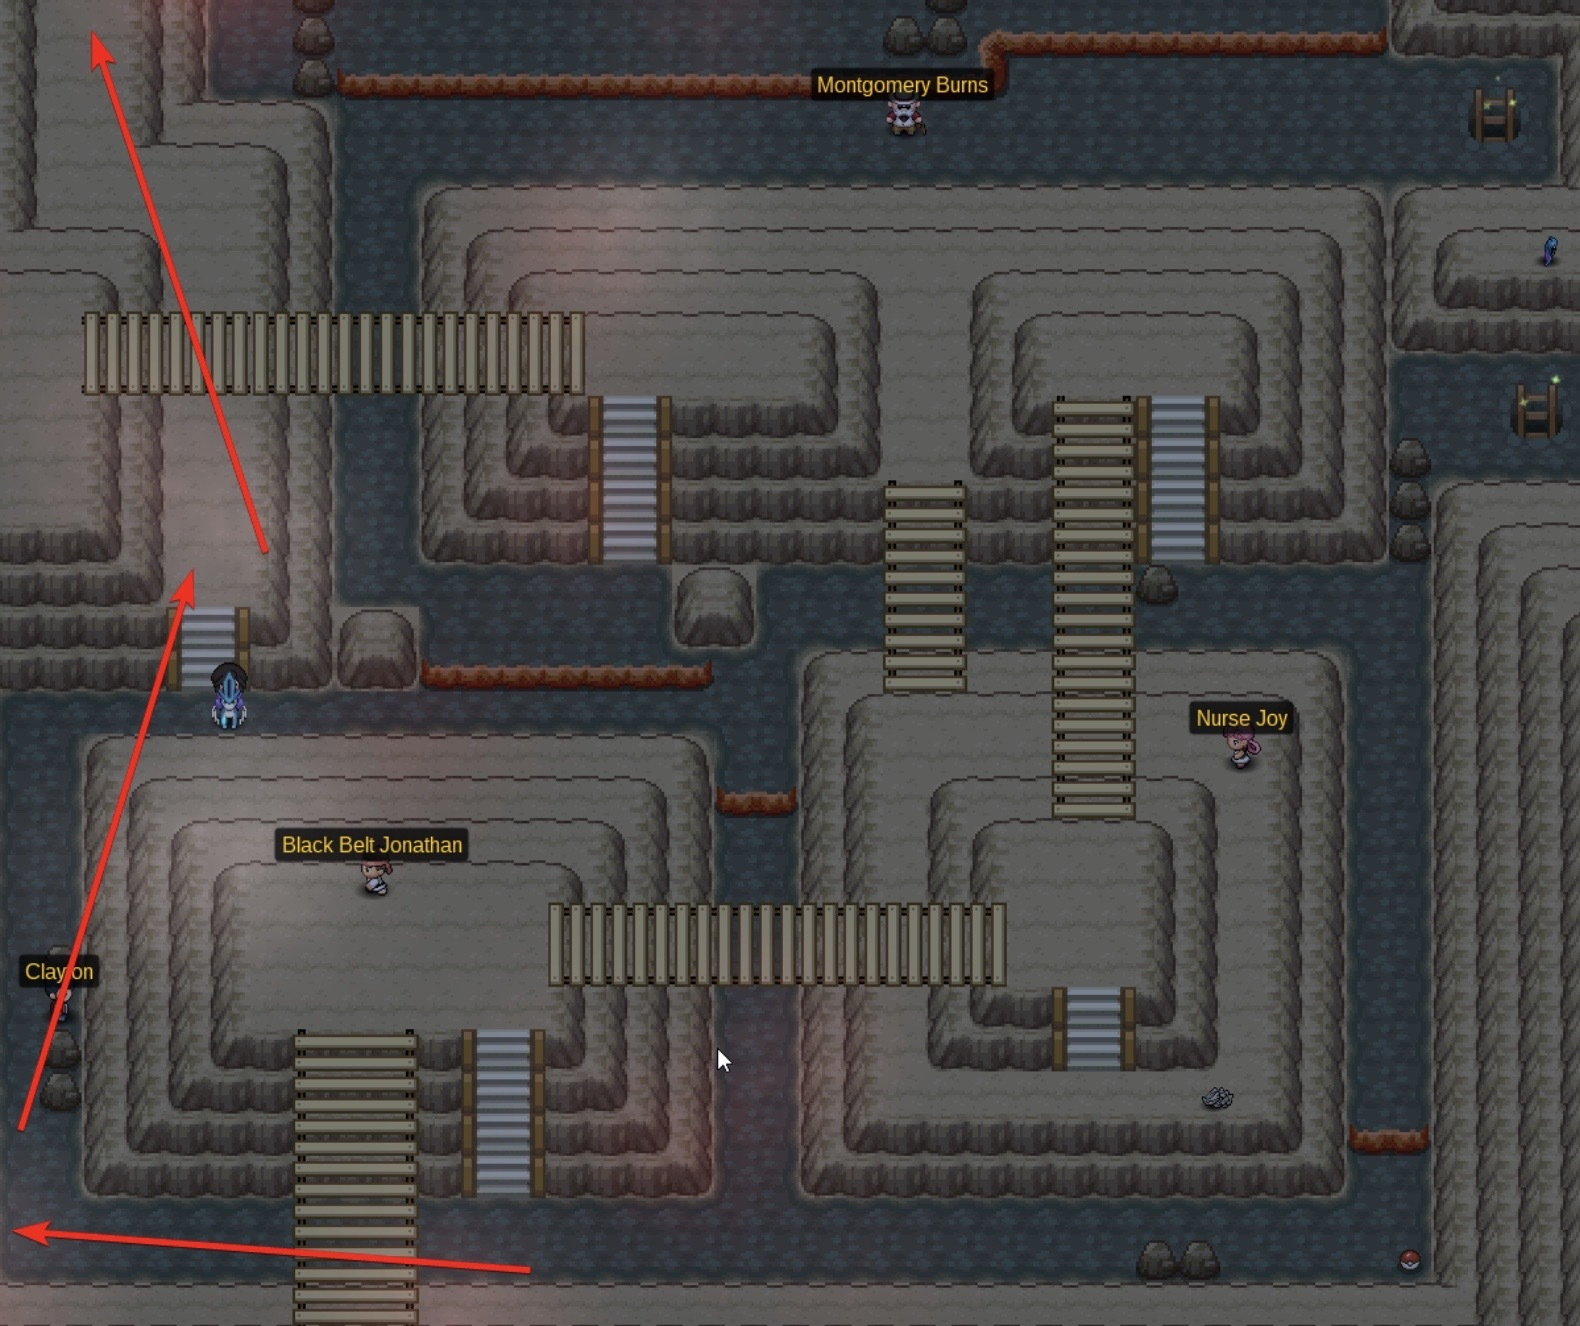
\includegraphics[width=\textwidth]{walkthrough/Sinnoh/victory-road-1}

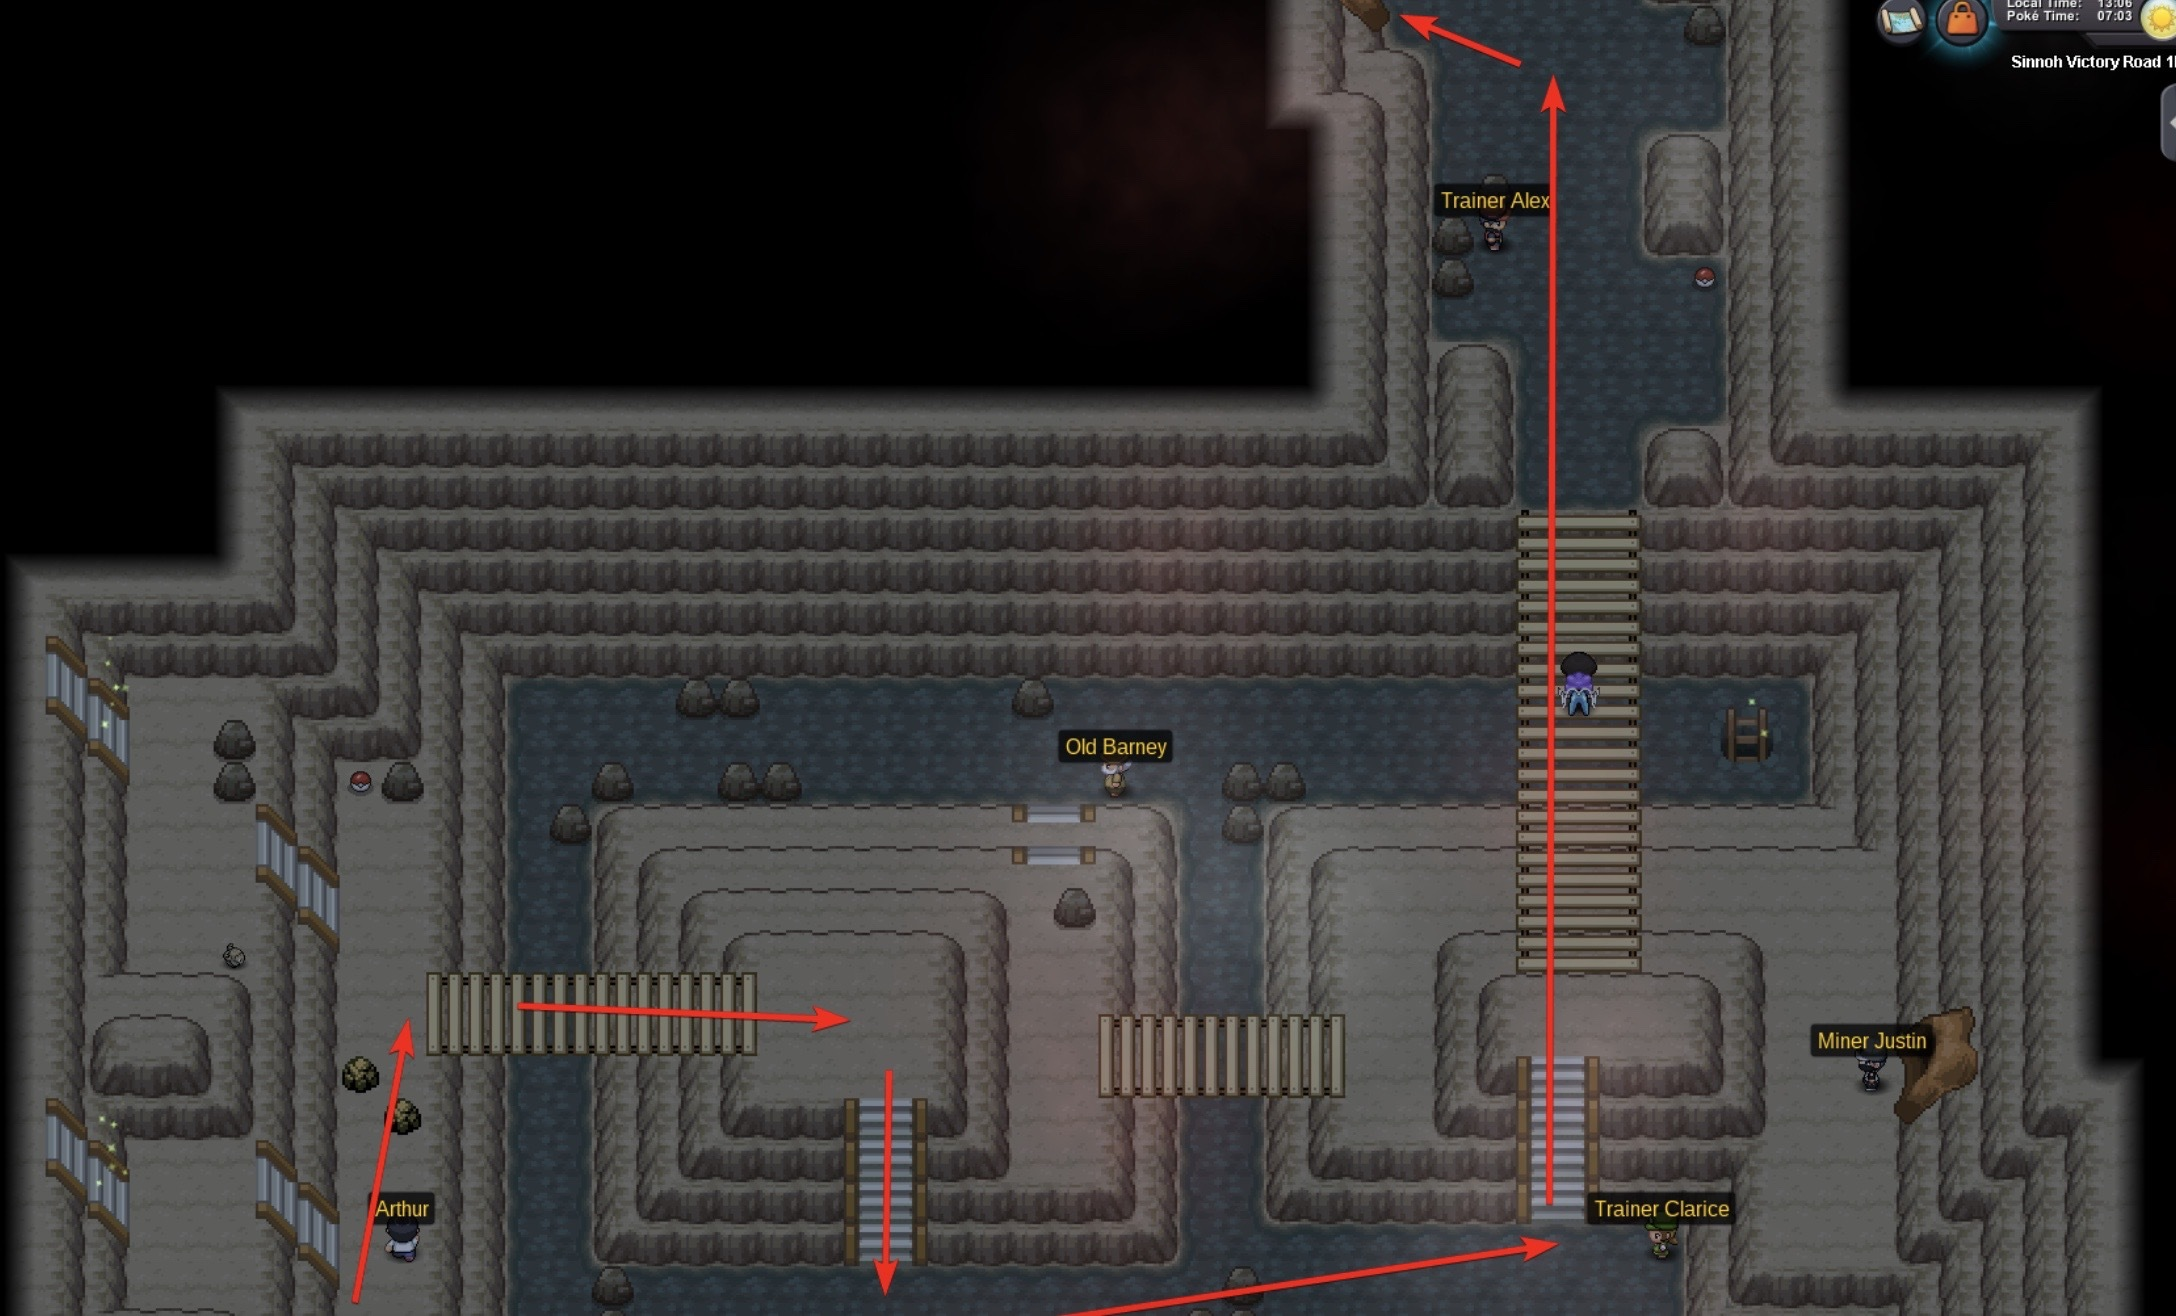
\includegraphics[width=\textwidth]{walkthrough/Sinnoh/victory-road-2}

\input{routes/Sinnoh/Sinnoh_Victory_Road_1F/Wild_Pokémon_(Sinnoh_Victory_Road_1F)}
\input{routes/Sinnoh/Sinnoh_Victory_Road_1F/Wild_Pokémon_(Sinnoh_Victory_Road_2F)}
% \input{routes/Sinnoh/Sinnoh_Victory_Road_1F/Wild_Pokémon_(Sinnoh_Victory_Road_B1F)}
% \input{routes/Sinnoh/Sinnoh_Victory_Road_1F/Wild_Pokémon_(Sinnoh_Victory_Road_B1F_Deep)}
\input{routes/Sinnoh/Sinnoh_Victory_Road_1F/Wild_Pokémon_(Sinnoh_Victory_Road_B1F_Deep_Entrance)}
\input{routes/Sinnoh/Sinnoh_Victory_Road_1F/Wild_Pokémon_(Sinnoh_Victory_Road_B1F_Deep_Exit)}
\begin{longtable}{|| l l l l ||}%
\hline%
&Razor Claw&x 1&Not respawnable\\%
\multicolumn{4}{||m{\textwidth}||}{In the south-east corner of 1F.}%
\hline%
&Ultra Ball&x 3&Not respawnable\\%
\multicolumn{4}{||m{\textwidth}||}{In the north-west corner of 1F.}%
\hline%
&Full Heal&x 1&Not respawnable\\%
\multicolumn{4}{||m{\textwidth}||}{Near the nothern exit, in front of Trainer Alex in 1F.}%
\hline%
&Max Potion&x 2&Not respawnable\\%
\multicolumn{4}{||m{\textwidth}||}{At the very end of the south-east path in 2F. Requires Rock Smash.}%
\hline%
&Zinc&x 1&Not respawnable\\%
\multicolumn{4}{||m{\textwidth}||}{In the south-west corner of 2F. Requires Rock Smash.}%
\hline%
&Max Repel&x 1&Not respawnable\\%
\multicolumn{4}{||m{\textwidth}||}{Hidden item. On the wall block adjacent to the rock smash rocks in the south-east corner, north-east from Psychic Bryce in 2F. Requires Rock Smash.}%
\hline%
&Rare Candy&x 1&Not respawnable\\%
\multicolumn{4}{||m{\textwidth}||}{Hidden item. On the rock one tile north of the northmost rock smash rock in the south-east path of 2F. Requires Rock Smash.}%
\hline%
&Max Elixir&x 1&Not respawnable\\%
\multicolumn{4}{||m{\textwidth}||}{Across the water from Fakuman, in the middle of B1F.}%
\hline%
&Pearl&x 1&Not respawnable\\%
\multicolumn{4}{||m{\textwidth}||}{Hidden item. From the south-westmost ladder, on the westmost accessible small rock before going down the stairs in B1F.}%
\hline%
&Calcium&x 1&Not respawnable\\%
\multicolumn{4}{||m{\textwidth}||}{Hidden item. On the small rock Black Belt Velskulz is running around near the north-west stairs of B1F.}%
\hline%
&Full Restore&x 1&Not respawnable\\%
\multicolumn{4}{||m{\textwidth}||}{In the north-west corner of B1F Deep. Requires Rock Smash.}%
\hline%
&Ether&x 2&Not respawnable\\%
\multicolumn{4}{||m{\textwidth}||}{In the middle of the northern body of water at the end of the south-east path in B1F Deep.}%
\hline%
&HP Up&x 1&Not respawnable\\%
\multicolumn{4}{||m{\textwidth}||}{In the west corner of the rock maze in the middle of B1F Deep.}%
\hline%
&Big Pearl&x 1&Not respawnable\\%
\multicolumn{4}{||m{\textwidth}||}{Hidden item. After entering the maze part from the south, follow the path north, west, north, east, then go south one tile, on the rock to the east in B1F Deep. Hinted by Mrs. Cherry.}%
\hline%
&Leftovers&x 1&Not respawnable\\%
\multicolumn{4}{||m{\textwidth}||}{Hidden item. After entering the maze part from the center, follow the path north, west one tile, north, west, south, west, north, on the rock to the north in B1F Deep.}%
\hline%
\endhead%
\hline%
\caption{Items in Sinnoh Victory Road 1F}%
\label{tab:SinnohVictoryRoad1FItems}%
\end{longtable}

\subsubsection{Sinnoh Elite Four}

\thispagestyle{empty}
\listoffigures
\listoftables
\newpage
\pagenumbering{arabic}

\end{document}
